% CVPR 2027 Paper Template; see https://github.com/cvpr-org/author-kit

%%%%%%%%% SIMULATED PAPER SWITCH
% \simulatedpaper builds the completed, evaluation-only paper from sim/. That version contains PROJECTED numbers
% (each one is wrapped in \simnum{...} in the source). It is for automated paper-scoring tools only.
% Without \simulatedpaper, the paper builds from sec/ exactly as before; nothing in sim/ is read.
% \showsimulated (only with \simulatedpaper) prints every projected number in red.
% After you change a switch, run: pdflatex, bibtex, pdflatex, pdflatex.
\newif\ifsimulatedpaper \newcommand{\simulatedpaper}{\simulatedpapertrue}
\newif\ifshowsimulated  \newcommand{\showsimulated}{\showsimulatedtrue}
% \simulatedpaper
% \showsimulated

\documentclass[10pt,twocolumn,letterpaper]{article}

%%%%%%%%% PAPER TYPE  - PLEASE UPDATE FOR FINAL VERSION
% \usepackage{cvpr}              % To produce the CAMERA-READY version
\usepackage[review]{cvpr}      % To produce the REVIEW version
% \usepackage[pagenumbers]{cvpr} % To force page numbers, e.g. for an arXiv version

% Import additional packages in the preamble file, before hyperref
%% This file contains a number of tweaks that are typically applied to the main document.
%% They are not enabled by default, but can be enabled by uncommenting the relevant lines.


%%
%% Official support for 2-column teaser figure
%%
\usepackage{cuted} %< for strip environment

%%
%% For auto-referencing of figures (see fig/teaser.tex and \label{} therein) 
%%
\usepackage{currfile} %< for \currfilebase macro

%%
%% caption and (global) spacing overrides
%%
\usepackage{caption} %< for "\captionof" commands (teaser)
% \setlength{\abovecaptionskip}{.5em} % space above caption
% \setlength{\belowcaptionskip}{1em} % space below caption

%%
%% Inline annotations; for predefined colors, refer to "dvipsnames" in the xcolor package:
%% https://tinyurl.com/overleaf-colors
%%
\newcommand{\red}[1]{{\color{red}#1}}
\newcommand{\todo}[1]{{\color{red}#1}}
\newcommand{\TODO}[1]{\textbf{\color{red}[TODO: #1]}}
%%
%% Disable for camera ready / submission by uncommenting these lines:
%%
% \renewcommand{\TODO}[1]{}
% \renewcommand{\todo}[1]{#1}

%%
%% Work harder in optimizing text layout. Typically shrinks text by 1/6 of page, enable
%% it at the very end of the writing process, when you are just above the page limit.
%%
% \usepackage{microtype}

%%
%% Fine-tune paragraph spacing.
%%
% \renewcommand{\paragraph}[1]{\vspace{.5em}\noindent\textbf{#1.}}

%%
%% Globally adjusts space between figure and caption.
%%
% \setlength{\abovecaptionskip}{.5em}

%%
%% Allows "the use of \paper to refer to the project name"
%% with automatic management of space at the end of the word.
%%
% \usepackage{xspace}
% \newcommand{\paper}{ProjectName\xspace}

%%
%% Commonly used math definitions.
%%
% \DeclareMathOperator*{\argmin}{arg\,min}
% \DeclareMathOperator*{\argmax}{arg\,max}

%%
%% Tighten underline.
%%
% \usepackage{soul}
% \setuldepth{foobar}

%%
%% Reconfigure paragraph (tweaks spacing)
%%

%%
%% Project additions (TALON), loaded before hyperref as the kit asks.
%%
% Workaround for lineno v5.7 (TeX Live 2026) with LaTeX >= 2025-06: its new column hook tags the wrong column,
% so right-column line numbers land in the gutter on top of the text. Restore lineno's pre-2025 column tagging.
\makeatletter
\@ifpackagelater{lineno}{2025/06/01}{%
  \RemoveFromHook{build/column/before}[lineno]%
  \AtBeginDocument{%
    \def\@LN@makecol{%
      \@LN@orig@makecol
      \setbox\@outputbox\vbox{%
        \boxmaxdepth\@maxdepth
        \protected@write\@auxout{}{\string\def\string\@LN@column{\if@firstcolumn1\else2\fi}}%
        \box\@outputbox}}}%
}{}
\makeatother

\usepackage{amsthm}
\usepackage{tikz}
\usepackage{algorithm}
\usepackage[noend]{algpseudocode}   % no "end for"/"end if" lines (DDPM / CLRS style)
\algrenewcommand\algorithmicrequire{\textbf{Input:}}
\algrenewcommand\algorithmicensure{\textbf{Output:}}
\algrenewcommand\algorithmicindent{1em}
\usetikzlibrary{arrows.meta, positioning, fit, backgrounds, calc, shapes.geometric, shapes.callouts}

% Propositions: plain run-in heads without a frame and without LaTeX list machinery. A tcolorbox frame made each
% proposition an unbreakable block, which the kit's \flushbottom turned into large white gaps. A list-based
% theorem (amsthm or \newtheorem) can lose its head into the page corner under the review-mode line numbering.
\newcounter{proposition}
\NewDocumentEnvironment{proposition}{o}
  {\par\addvspace{\topsep}\refstepcounter{proposition}\noindent
   \textbf{Proposition~\theproposition}\IfValueT{#1}{ (#1)}\textbf{.}\ \itshape\ignorespaces}
  {\par\addvspace{\topsep}}
\newtheorem{lemma}{Lemma}
\newcommand{\name}{TALON\xspace}
\newcommand{\one}{\mathbf{1}}
\DeclareMathOperator*{\argmax}{arg\,max}
\DeclareMathOperator*{\argmin}{arg\,min}

% TikZ colours used by the overview figure (fig/overview.tex)
\definecolor{orxblue}{HTML}{0072B2}
\definecolor{orxorange}{HTML}{E69F00}
\definecolor{orxgreen}{HTML}{009E73}
\definecolor{orxred}{HTML}{D55E00}
\definecolor{orxpurple}{HTML}{CC79A7}
\definecolor{orxsky}{HTML}{56B4E9}

\newcommand{\ayush}[1]{\textcolor{purple}{[Ayush: #1]}}
\newcommand{\fan}[1]{\textcolor{blue}{[Fan: #1]}}
\newcommand{\francis}[1]{\textcolor{orange}{[Francis: #1]}}
\ifsimulatedpaper% Additions for the simulated paper. main.tex reads this file only when \simulatedpaper is set.
% \simnum{...} marks a PROJECTED number (not measured). It prints the number unchanged, or in red with \showsimulated.
% List every projected number:  grep -n -o 'simnum{[^}]*}' sim/*.tex
%
% How each projection was made (2026-11-13). Replace them with measurements as the runs finish.
%  Table 1, InternVL3.5-4B rows Top-K (w/ pruning), Q-Frame, TALON: additive model. Accuracy = the method's
%    Qwen3-VL-8B accuracy + the mean InternVL-minus-Qwen shift of the three measured baselines (QuoTA, FOCUS,
%    AdaAlloc) in that column. TFLOPs = the method's Qwen TFLOPs x (FOCUS InternVL / FOCUS Qwen) in that column.
%  Table 2, w/o water-filling: the 300-question ablation subset (proportional 74.0 vs TALON 77.3) with the
%    per-duration gaps shrunk by 0.6, the ratio seen for "w/o text allocation" between that subset and the full set.
%  Table 3, w/o carried allocation: compute = Q-Frame's measured cost in standard multi-turn chat at the same
%    per-turn budget (about 640 TFLOPs per conversation); accuracy placed between the two measured rows.
%  Table 1, VideoRAG and VideoRAG + TALON rows: ASSUMED, no measurement exists. Base set near Top-K (w/ pruning);
%    the TALON gain set near the gain over Top-K in the embedding-based rows; TFLOPs set near the other rows.
%  The appendix is a separate document; sim/X_suppl.tex (proof drafts) is not read by main.tex.
\newcommand{\simnum}[1]{\ifshowsimulated\textcolor{red}{#1}\else#1\fi}
\fi

% It is strongly recommended to use hyperref, especially for the review version.
% hyperref with option pagebackref eases the reviewers' job.
% Please disable hyperref *only* if you encounter grave issues, 
% e.g. with the file validation for the camera-ready version.
%
% If you comment hyperref and then uncomment it, you should delete *.aux before re-running LaTeX.
% (Or just hit 'q' on the first LaTeX run, let it finish, and you should be clear).
\definecolor{cvprblue}{rgb}{0.21,0.49,0.74}
\usepackage[pagebackref,breaklinks,colorlinks,allcolors=cvprblue]{hyperref}


\def\confName{CVPR}
\def\confYear{2027}

%%%%%%%%% TITLE - PLEASE UPDATE
\title{Moving from Frames to Tokens for Video Retrieval-Augmented Generation}

%%%%%%%%% AUTHORS - PLEASE UPDATE (hidden in review mode)
\author{Anonymous CVPR submission}

\begin{document}
\maketitle
\ifsimulatedpaper
\begin{abstract}
Video retrieval-augmented generation (RAG) answers a question about a long video by passing the most relevant frames
to a vision-language model (VLM). Existing systems, however, operate at the frame level: every retrieved frame enters
the VLM at the same token cost, although frames differ widely in relevance and the value of a frame saturates with its
token count. We present \name, a plug-and-play token allocation framework that moves video RAG from frames to tokens.
\name formulates evidence selection as a budgeted optimization over the token count of every frame and transcript
segment, with a token value function fitted offline, and solves it by iterative water-filling, which attains a higher
objective than the fixed allocation rules of prior work. In multi-turn conversations, \name carries the allocation
across turns: it updates relevance with the attention of the VLM and prefills only the tokens that the KV cache lacks,
so that the cumulative prefill of a conversation provably stays bounded. On MLVU, LongVideoBench, and Video-MME with
two VLMs, \name improves accuracy by up to 4.2 points over compute-matched frame selection and token allocation
methods, and matches or exceeds the strongest prior method at roughly one third of its compute. On MT-Video-Bench,
\name reduces the compute of a conversation by up to 5.2$\times$ at comparable accuracy.
\end{abstract}

\section{Introduction}
\label{sec:intro}

\begin{figure}[t]
  \centering
  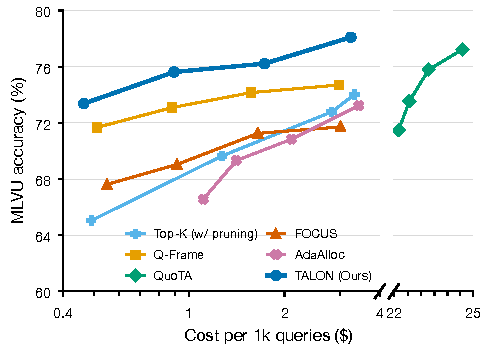
\includegraphics[width=\linewidth]{fig/budget_curve.pdf}
  \caption{\textbf{Accuracy against cost on MLVU} (Qwen3-VL-8B). Each line traces one method across token budgets
    from 1,536 to 12,288. Cost prices the input tokens of 1,000 queries at OpenRouter rates. The scorer calls of QuoTA place it beyond the axis break.}
  \label{fig:budget}
\end{figure}

Vision-language models (VLMs) now answer open-ended questions about
videos~\cite{bai2025qwen3vl,wang2025internvl35}, and the videos of practical interest are long. Applications such as
video analytics over camera feeds~\cite{yan2025ava} and search over lectures, meetings, and broadcasts pose questions whose evidence occupies a few seconds of a video that
lasts from minutes to hours~\cite{fu2024videomme,zhou2024mlvu,wu2024longvideobench}.

Processing every frame of such a video is impractical: an hour of video at one frame per second yields millions of
visual tokens, far beyond the context window of current VLMs.
Existing systems, therefore, widely resort to retrieval-augmented generation (RAG). They index the video offline,
either by embedding its frames and transcript~\cite{luo2024videorag,jeong2025videorag} or by building a graph over
its clips and entities~\cite{ren2025videorag,shen2025vgent,yan2025ava,yang2026g2frag,chen2026memdreamer,yan2026ecrag}, and supply the VLM with only the evidence
retrieved for each query.

Both forms of RAG, however, have limitations. Graph-based RAG attains high accuracy, but must caption and link
the whole video before the first question arrives, a cost that is often wasted because users query a video
sporadically. Embedding-based RAG is lightweight, but it operates at the frame level: it admits the top-$K$ frames
and passes each of them to the VLM at the same token cost. This uniform cost is wasteful, since the relevance of the
retrieved frames is highly uneven, and the value of a frame saturates with its token count (\cref{fig:value}), so
that most tokens of a frame are better spent on other frames. Token
compression~\cite{chen2024fastv,yang2024visionzip,shen2024longvu} mitigates this issue, but compresses every frame
independently, and recent query-aware methods vary the token count of frames only with fixed rules, such as
resolution tiers~\cite{zhang2025qframe} or shares proportional to relevance~\cite{luo2025quota}. None of these
methods solves for the division of a global token budget across frames, although a different division could reveal
useful evidence in other frames.

These limitations motivate us to move video RAG from frames to tokens. We present \name, a plug-and-play
\textbf{T}oken \textbf{AL}locati\textbf{ON} framework that is placed between a retriever and a VLM, and decides how
many tokens each retrieved frame and transcript segment receives. \name formulates this decision as one optimization
problem, which maximizes the relevance-weighted value of the evidence subject to a token budget.

Realizing this formulation raises two challenges. The first is to value tokens and to solve the allocation
efficiently. The Token Scheduler of \name learns a \textit{token value} function offline, discounts frames that
duplicate others already shown, and lets frames and transcript segments compete for the same budget. It solves the
resulting problem by iterative water-filling, and we derive the optimal allocation, which the
allocation rules of prior work do not attain. The second challenge arises in multi-turn conversations, where re-allocating tokens
for every question invalidates the KV cache that LLM serving systems reuse across
turns~\cite{kwon2023vllm,zheng2024sglang}. \name instead carries the allocation across turns: it updates the
relevance of cached frames with the attention of the VLM, and prefills only the tokens that the cache lacks, so that
the cumulative prefill of evidence tokens provably stays bounded.

We evaluate \name on MLVU, LongVideoBench, and Video-MME with two VLMs, and on the multi-turn MT-Video-Bench. At the
same budget of 12,288 tokens, \name improves the accuracy of Qwen3-VL-8B by 2.2 to 4.2 points over retrieval with
uniform token pruning, and matches or exceeds QuoTA, the strongest baseline, which requires 2.8--3.4$\times$ more
compute. With a quarter of the budget, \name is more accurate on MLVU than Q-Frame, FOCUS, and AdaAlloc at the full
budget (\cref{fig:budget}), and its gains carry over to graph-based retrieval when paired with VideoRAG. In
conversations, it uses up to 5.2$\times$ less compute at comparable accuracy.

Our contributions are as follows:
\begin{itemize}
  \item We introduce \name, a plug-and-play framework that formulates video RAG as one budgeted token allocation
    over frames and transcript segments.
  \item We design the Token Scheduler, which combines a learned token value with iterative water-filling, and derive
    the optimal allocation of its objective, which the allocation rules of prior work do not attain.
  \item We extend token allocation to multi-turn conversations with KV-cache reuse and attention-updated
    relevance, and prove that the cumulative prefill of evidence tokens stays bounded.
\end{itemize}

\section{Related Work}
\label{sec:related}

\paragraph{Video retrieval augmented generation.}
RAG grounds generation in retrieved evidence. For long videos, Video-RAG~\cite{luo2024videorag} augments a VLM with
visually aligned auxiliary texts, such as speech transcripts, on-screen text, and detected objects, retrieved for each
query, and VideoRAG~\cite{jeong2025videorag} retrieves whole videos from a corpus as external knowledge. A second line
of work structures the index. VideoRAG~\cite{ren2025videorag} builds a graph-based knowledge index across videos,
Vgent~\cite{shen2025vgent} represents a video as a graph of clips that preserves their semantic and temporal
dependencies, followed by a structured reasoning step that filters retrieval noise, and AVA~\cite{yan2025ava} indexes a
video as an event knowledge graph that an agent searches. Other systems add spatio-temporal
structure~\cite{fu2026videostir} or temporal alignment~\cite{cao2025tvrag} to retrieval, and
\citet{lee2026rethinking} benchmark retrieval and generation separately.
These systems, however, focus on what to index and retrieve, and pass every retrieved item to the VLM at its full
cost. \name instead decides how many tokens each retrieved item receives, and can be placed after any of these
retrievers.

\paragraph{Keyframe selection.}
Most VLMs sample frames uniformly and therefore often miss the content that a query needs. Query-aware methods instead
select frames by jointly optimizing their relevance and temporal coverage~\cite{tang2025aks,peng2026qca}, by greedy
marginal utility~\cite{shi2026markey}, by learning to query informative combinations of
frames~\cite{yu2024framevoyager}, with the attention of a small VLM used as a selector~\cite{wang2026dafs}, or by
exploring clips as the arms of a bandit~\cite{zhu2026focus}. All of these methods, however, return a subset of frames,
each at the same token cost. \name instead treats the token count of each frame as a decision variable.

\paragraph{Token allocation across frames.}
Closest to our work are methods that vary the token count of frames. Q-Frame~\cite{zhang2025qframe} shows frames at
three resolutions according to their relevance rank, QuoTA~\cite{luo2025quota} assigns tokens in proportion to a
query-oriented frame score, and AdaptToken~\cite{qi2026adapttoken} distributes a global token budget over groups of
frames according to the response entropy of the VLM. Concurrent with our work, AdaAlloc~\cite{an2026adaalloc} lets the
VLM plan how to split the budget between sparse low-resolution frames and dense high-resolution frames; it became
public after the CVPR~2027 cutoff for prior work, and we include it in our comparisons for completeness. All of these
methods allocate with a fixed rule or a heuristic plan. \name instead derives the allocation as the solution of an
optimization problem with a learned token value, extends it to transcripts, and maintains it across the turns of a
conversation.

\paragraph{Token compression and KV-cache reuse.}
A complementary line of work reduces the tokens of a given input. FastV~\cite{chen2024fastv} and
VisionZip~\cite{yang2024visionzip} prune visual tokens by attention, ToMe~\cite{bolya2023tome} merges similar tokens
inside the vision encoder, and LongVU~\cite{shen2024longvu}, DyCoke~\cite{tao2024dycoke}, and
MARC~\cite{wu2026marc} compress video tokens by exploiting their temporal redundancy. For language models,
H$_2$O~\cite{zhang2023h2o} and StreamingLLM~\cite{xiao2024streamingllm} evict entries of the KV cache, and
ReKV~\cite{rekv2025} retrieves cached video KV entries for streaming question answering. These methods, however,
compress each frame or cache independently. \name uses a pruner only to realize a token count, decides the counts
jointly, and reuses cached tokens instead of evicting them.

\section{Method}
\label{sec:method}

\begin{figure*}[t]
  \centering
  \makebox[\linewidth][c]{% Overview figure (figure*, drawn at \textwidth = 17.46 cm). The Overleaf figure (fig/overview_v1.tex), refined:
% numbered stages with a one-line description each, single-turn inference only (no KV cache), less empty space,
% larger frames and text. Three stages left to right:
% (1) retrieval: video + subtitles -> retriever (with query q) -> relevance r_i over items in time order;
% (2) Token Scheduler (the contribution, the only accented stage): objective, value curves v_frame / v_text,
%     water-filling -> token plan b_i;
% (3) inference: frozen pruner keeps each frame's top-ranked tokens, the frozen VLM answers.
% Bar heights and the plan are illustrative, not measured. Frames: Video-MME video bepwr1-CNRU (illustration only).
% Tableau 10 (Stone, 2016): blue 4E79A7 and orange F28E2B on neutral greys; dark text on light fills only
\definecolor{ink}{HTML}{333333}%
\definecolor{arrowgray}{HTML}{6F6F6F}%
\definecolor{bandA}{HTML}{F4F5F7}%
\definecolor{bandB}{HTML}{EAF1F8}%
\definecolor{edgeB}{HTML}{4E79A7}%
\definecolor{bandC}{HTML}{F4F5F7}%
\definecolor{stepA}{HTML}{333333}%
\definecolor{stepB}{HTML}{4E79A7}%
\definecolor{stepC}{HTML}{333333}%
\definecolor{modelA}{HTML}{DCE6F1}%
\definecolor{modelC}{HTML}{DCE6F1}%
\definecolor{modelD}{HTML}{4E79A7}%
\definecolor{modelT}{HTML}{333333}%
\definecolor{flake}{HTML}{4E79A7}%
\definecolor{chipF}{HTML}{FFFFFF}%
\definecolor{chipD}{HTML}{A0A0A0}%
\definecolor{frm}{HTML}{4E79A7}%
\definecolor{txt}{HTML}{F28E2B}%
\definecolor{accA}{HTML}{4E79A7}%
% every color role: ink, arrowgray, bandA/B/C, edgeB, stepA/B/C, modelA/C/D/T, flake, chipF/D, frm, txt
\newcommand{\snowflake}[2]{%
  \begin{scope}[shift={#1}, line width=0.55pt, draw=flake, line cap=round]
    \foreach \a in {0,60,...,300}{\draw (0,0) -- (\a:#2);
      \draw (\a:0.55*#2) -- ++(\a+45:0.32*#2); \draw (\a:0.55*#2) -- ++(\a-45:0.32*#2);}
  \end{scope}}
% \items{width}{height scale}{v1/t1,...,v20/t20}: 20 items on one time axis; t = 1 marks a transcript event (light bar)
\newcommand{\items}[3]{%
  \foreach \v/\t [count=\i] in {#3} {
    \ifnum\t=1 \fill[txt] ({(\i-0.5)*#1/20-0.3*#1/20},0) rectangle ++({0.6*#1/20},{\v*#2});
    \else      \fill[frm]    ({(\i-0.5)*#1/20-0.3*#1/20},0) rectangle ++({0.6*#1/20},{\v*#2}); \fi}}
% \prunedframe{center}{image}{kept tokens out of 32}: a frame (1.0 cm) as an 8x4 token grid; dropped tokens greyed out.
% The keep order is one fixed ranking (centre first), so a frame at b tokens holds its top b tokens.
\newcommand{\prunedframe}[3]{%
  \node[inner sep=0pt] at (#1) {\includegraphics[width=1.0cm]{fig/frames/#2}};
  \begin{scope}[shift={($(#1)+(-0.5,-0.28125)$)}]
    \foreach \c [count=\k from 0] in {10,11,18,19,9,12,17,20,2,3,26,27,1,4,25,28,8,13,16,21,0,5,24,29,6,14,22,30,7,15,23,31} {
      \ifnum\k<#3\relax\else
        \pgfmathtruncatemacro{\cx}{mod(\c,8)}\pgfmathtruncatemacro{\cy}{int(\c/8)}
        \fill[white, opacity=0.85] (\cx*0.125,\cy*0.140625) rectangle ++(0.125,0.140625);
      \fi}
    \draw[ink!30, line width=0.15pt, xstep=0.125, ystep=0.140625] (0,0) grid (1.0,0.5625);
    \draw[ink!45, line width=0.3pt] (0,0) rectangle (1.0,0.5625);
  \end{scope}}
\newcommand{\txtchip}[1]{% transcript event: a short text chip
  \fill[txt!35, rounded corners=1pt] ($(#1)+(-0.42,-0.2)$) rectangle ++(0.84,0.4);
  \draw[txt!85!black, line width=0.5pt] ($(#1)+(-0.3,0.07)$) -- ++(0.6,0);
  \draw[txt!85!black, line width=0.5pt] ($(#1)+(-0.3,-0.07)$) -- ++(0.4,0);}
% \stage{x}{y}{number}{title}{one-line description}: numbered stage heading
\newcommand{\stage}[5]{%
  \node[circle, fill=#5, text=white, font=\sffamily\scriptsize\bfseries, inner sep=0pt, minimum size=0.4cm] at (#1+0.2,#2) {#3};
  \node[font=\sffamily\small\bfseries, text=#5, anchor=west, inner sep=0pt] at (#1+0.5,#2) {#4};}

\begin{tikzpicture}[font=\sffamily\footnotesize, text=ink, line width=0.6pt,
  card/.style={fill=white, draw=ink!18, line width=0.5pt, rounded corners=4pt, align=center, inner sep=3.5pt},
  arr/.style={-{Stealth[length=5pt, width=4pt]}, draw=arrowgray, line width=0.8pt},
  ax/.style={-{Stealth[length=3.5pt, width=3pt]}, draw=ink!55, line width=0.5pt},
  axl/.style={font=\sffamily\scriptsize, text=ink!70},
  desc/.style={font=\sffamily\scriptsize, text=ink!65, anchor=north west, inner sep=0pt, align=left},
  elbl/.style={font=\sffamily\scriptsize, text=ink!75, inner sep=1.5pt},
  model/.style={fill=modelC, draw=modelD, text=modelT, line width=0.5pt, rounded corners=3pt, align=center,
    minimum height=0.62cm, inner xsep=5pt, font=\sffamily\footnotesize},
  qa/.style={fill=chipF, draw=chipD, line width=0.5pt, rounded corners=3pt, align=left,
    inner sep=3pt, font=\sffamily\scriptsize}]

% ---------------- layout ----------------
% Top row: (1) Retrieval -> (2) Allocation; bottom row: (3) Inference, left to right. Stages connect box to box
% (r_i, b_i). Q sits inside Retrieval and A inside Inference; nothing is outside the stage boxes.
\fill[rounded corners=6pt, bandA] (0,2.0) rectangle (7.5,5.3);
\fill[rounded corners=6pt, bandB] (8.0,2.0) rectangle (17.4,5.3);
\draw[rounded corners=6pt, edgeB, line width=0.6pt] (8.0,2.0) rectangle (17.4,5.3);
\fill[rounded corners=6pt, bandC] (0,0) rectangle (17.4,1.6);
\stage{0.12}{5.02}{1}{Retrieval}{stepA}
\stage{8.12}{5.02}{2}{Allocation}{stepB}
\stage{0.12}{1.3}{3}{Inference}{stepC}
\draw[arr] (7.5,3.65) -- node[elbl, above] {$r_i$} (8.0,3.65);
\draw[arr] (12.7,2.0) -- node[elbl, right] {$b_i$} (12.7,1.6);

% ---------------- (1) retrieval ----------------
\fill[ink!88, rounded corners=1pt] (0.2,3.85) rectangle (7.3,4.75);
\foreach \x in {0.28,0.48,...,7.2} {\fill[white] (\x,4.65) rectangle ++(0.1,0.06); \fill[white] (\x,3.89) rectangle ++(0.1,0.06);}
\foreach \k in {1,...,5} {\node[inner sep=0pt] at ({0.91+(\k-1)*1.42},4.3) {\includegraphics[width=1.2cm]{fig/frames/frame\k.jpg}};}
\fill[txt!35, rounded corners=1pt] (0.2,3.57) rectangle (7.3,3.77);
\foreach \x/\l in {0.5/1.0, 1.9/0.8, 3.1/1.2, 4.7/0.9, 6.0/0.9} {\draw[txt!85!black, line width=0.5pt] (\x,3.67) -- ++(\l,0);}
\node[qa] (q) at (1.0,2.75) {\textbf{Q:} Color of\\the last car?};
\node[model, fill=modelA] (ret) at (2.95,2.75) {Retriever\hspace{0.12cm}};
\snowflake{($(ret.north east)+(-0.14,-0.14)$)}{0.075}
\draw[arr] (q.east) -- (ret.west);
\draw[arr] (2.95,3.55) -- (ret.north);
\begin{scope}[shift={(4.25,2.42)}]
  \draw[ax] (0,0) -- (3.05,0); \draw[ax] (0,0) -- (0,1.0);
  \node[axl, anchor=west] at (0.06,0.93) {$r_i$};
  \node[axl, anchor=north] at (1.5,-0.02) {frame \#};
  \items{2.95}{1.4}{.04/0,.06/0,.30/0,.52/0,.20/1,.40/0,.10/0,.05/0,.04/0,.36/1,
                   .06/0,.22/0,.30/0,.42/1,.34/0,.26/0,.08/0,.18/1,.05/0,.03/0}
\end{scope}
\draw[arr] (ret.east) -- (4.15,2.75);

% ---------------- (2) allocation ----------------
\node[font=\sffamily\scriptsize] at (12.7,4.5) {$\max\limits_{\mathbf b}\ \sum_i r_iv_i(b_i)-\eta\sum_{i\neq j}s_{ij}\,v_i(b_i)\,v_j(b_j)\qquad\text{s.t.}\ \ \sum_i b_i\le B$};
\begin{scope}[shift={(8.75,2.42)}]
  \draw[ax] (0,0) -- (3.2,0); \draw[ax] (0,0) -- (0,1.6);
  \node[axl, anchor=west] at (0.06,1.5) {$v(b)$};
  \node[axl, anchor=north] at (1.6,-0.02) {$b$};
  \draw[txt, line width=1.1pt, domain=0.02:8, samples=60] plot ({0.37*\x}, {1.45*((2^\x-1)^0.841)/(((2^\x-1)^0.841)+3.44)});
  \draw[frm, line width=1.1pt, domain=0.02:8, samples=60] plot ({0.37*\x}, {1.35*((2^\x-1)^0.841)/(((2^\x-1)^0.841)+7.73)});
  \node[font=\sffamily\scriptsize, text=txt!80!black, anchor=south west, inner sep=1pt] at (3.0,1.35) {$v_{\text{text}}$};
  \node[font=\sffamily\scriptsize, text=frm, anchor=north west, inner sep=1pt] at (3.0,1.2) {$v_{\text{frame}}$};
\end{scope}
\draw[arr] (12.75,3.2) -- (13.45,3.2);
\begin{scope}[shift={(13.85,2.42)}]
  \draw[ax] (0,0) -- (3.3,0); \draw[ax] (0,0) -- (0,1.6);
  \node[axl, anchor=west] at (0.06,1.5) {$b_i$};
  \node[axl, anchor=north] at (1.6,-0.02) {frame \#};
  \items{3.2}{1.9}{0/0,0/0,.438/0,.688/0,.25/1,.531/0,0/0,0/0,0/0,.5/1,
                   0/0,.25/0,.344/0,.5/1,.406/0,.312/0,0/0,.25/1,0/0,0/0}
\end{scope}

% ---------------- (3) inference ----------------
% the frozen pruner is a container that holds its output: the frames at their token counts and the text events
\node[model, minimum width=9.4cm, minimum height=1.0cm] (pr) at (7.3,0.7) {};
\node[font=\sffamily\footnotesize, text=modelT, align=center] at (3.4,0.7) {Token\\pruner};
\snowflake{($(pr.north east)+(-0.14,-0.14)$)}{0.075}
\prunedframe{4.95,0.7}{frame1.jpg}{6}
\txtchip{6.15,0.7}
\prunedframe{7.35,0.7}{frame3.jpg}{22}
\prunedframe{8.55,0.7}{frame4.jpg}{12}
\txtchip{9.75,0.7}
\prunedframe{10.95,0.7}{frame5.jpg}{32}
\node[model, minimum width=2.4cm, minimum height=1.0cm] (vlm) at (14.0,0.7) {VLM};
\snowflake{($(vlm.north east)+(-0.14,-0.14)$)}{0.075}
\node[qa] (ans) at (16.4,0.7) {\textbf{A:} Blue};
\draw[arr] (pr.east) -- (vlm.west);
\draw[arr] (vlm.east) -- (ans.west);
\end{tikzpicture}
}
  \caption{\textbf{\name overview.} (1)~A retriever scores the relevance of every frame and transcript segment to the query. (2)~The Token Scheduler divides the token budget across them by maximizing their relevance-weighted token value, which it solves by iterative water-filling. (3)~A frozen token pruner keeps the allocated number of tokens of each frame, and the frozen VLM answers from the resulting storyboard.}
  \label{fig:overview}
\end{figure*}

\subsection{Overview and Problem Formulation}
\label{sec:overview}

Frame-level RAG answers a user query $q$ about a video $V$ by passing the top-$K$ most semantically relevant frames to a VLM~\cite{ren2025videorag,shen2025vgent,tang2025aks}. Let $f_1, \dots, f_N$ be frames sampled uniformly from $V$, and let $r(f_i\mid q)$ denote the relevance of $f_i$ to $q$. Mathematically, frame-level RAG makes a binary admit-or-reject decision for each frame, subject to a budget of $K$ frames, so as to maximize the total relevance of the admitted frames. It is therefore naturally modeled as an integer linear program:
\begin{equation}
  \max_{\mathbf{x} \in \{0,1\}^N} \sum_{i=1}^{N} r(f_i\mid q)\, x_i \qquad \text{s.t.} \quad \sum_{i=1}^{N} x_i \le K,
  \label{eq:topk}
\end{equation}
where $f_i$ is passed to the VLM if $x_i=1$ and dropped if $x_i=0$, and
\begin{equation}
  r(f_i\mid q)=\operatorname{softmax}_i\big(\cos(f_i,q)\big)
  \label{eq:rel}
\end{equation}
is the cosine similarity between the image embedding of $f_i$ and the text embedding of $q$ (e.g., CLIP~\cite{radford2021clip}), normalized across frames. We lift this frame-level objective to a multimodal token-level objective that defines \textit{how} tokens should be valued, and prove that our solution strictly outperforms prior token allocation rules on it (\cref{sec:allocation}). In multi-turn conversations, however, naively re-allocating tokens at every turn is inefficient and breaks prefix caching~\cite{kwon2023vllm,zheng2024sglang}, a standard feature of LLM inference. 

At its core, \name carries the allocation across turns, reusing the KV cache and updating relevance with the attention of the VLM. This improves both efficiency and accuracy, and we prove that the cumulative prefill stays bounded however long the conversation lasts, owing to the design of our token pruner (\cref{sec:multiturn}).


\subsection{Token Scheduler}
\label{sec:allocation}

\begin{figure}[t]
  \centering
  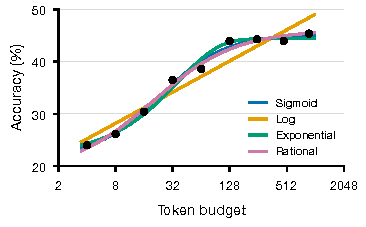
\includegraphics[width=0.75\linewidth]{fig/value_curve.pdf}
  \caption{\textbf{Token value saturates.} Accuracy of the VLM on calibration questions when every frame is shown with the same number of tokens (dots), with four concave families fitted to the measurements. Accuracy rises steeply at low token counts and flattens well before the native token count of a frame. \name uses the rational form.}
  \label{fig:value}
\end{figure}

Moving from frame-level to token-level RAG replaces the binary decision $x_i$ by the number of tokens $b_i$ allocated to frame $f_i$, and the frame budget $K$ by a token budget $B$. This formulation, however, raises two key questions: (i) how much is a frame worth at a given token count, and (ii) how should the relevance of a frame change once similar frames already receive tokens? 

\name answers both in its Token Scheduler, which computes the token allocation: the first with a token value function that is fitted offline and updated online and asynchronously to serving, and the second by conditioning relevance on the current allocation. We formulate both for frames and then extend them to the transcript of the video.

\paragraph{Pruning Frames and Transcripts to a Token Count.}
Allocating $b_i$ tokens to a frame requires a way to show the frame with any number of tokens. \name passes each frame through the vision encoder of the VLM once, ranks its output tokens by the attention they receive within the encoder, and keeps the top $b_i$, following attention-based token pruning~\cite{yang2024visionzip,chen2024fastv}. Transcript events are pruned in the same way.

\paragraph{Capturing Token Value.}
Intuitively, the token count of a frame acts as its effective resolution: with few tokens, the VLM perceives only the coarse structure of the frame, whereas with more tokens it also perceives fine detail, such as on-screen text. How this added detail translates into accuracy, however, depends on the VLM and the videos it serves. \name therefore learns a \textit{token value} function by logistic regression on the logarithm of the token count $b$ of a frame,
\begin{equation}
  v(b)=\sigma\big(\log b-\log\tau\big)=\frac{b}{b+\tau} ,
  \label{eq:curve}
\end{equation}
where $\tau$ is the token count at which a frame reaches half of its full value. \name fits $\tau$ by maximum likelihood offline, on calibration video--query pairs with the tokens per frame varied uniformly (\cref{fig:value}), and updates it online from feedback on answered queries (e.g., accuracy, user feedback). The form has a single parameter, so the fit is stable with few calibration samples. Weighting the value of each frame by its relevance gives the token-level objective
\begin{equation}
  \max_{\mathbf b}\ \sum_{i}r(f_i\mid q)\,v(b_i)\qquad\text{s.t.}\quad\sum_{i}b_i\le B .
  \label{eq:relevance}
\end{equation}

\paragraph{Incorporating Frame Diversity.}
The objective above, however, scores every frame in isolation. Consecutive frames often show the same content, so it may spend tokens on near-duplicate frames, each of which $v$ credits in full, even though a second copy adds little once the first is shown. \name therefore conditions the relevance of a frame on the current allocation as well as the query, discounting it by its cosine similarity to every frame, weighted by the value of that frame:
\begin{equation}
  r(f_i\mid q,\mathbf b)=r(f_i\mid q)-\eta\sum_{j}\cos(f_i,f_j)\,v(b_j) ,
  \label{eq:cond}
\end{equation}
where $\eta$ sets the strength of the discount. The similarity reuses the frame embeddings that retrieval already computes, so the discount adds no model call. A frame that duplicates a frame shown with many tokens thus loses most of its relevance, while one that duplicates a dropped frame keeps it. \name then solves
\begin{equation}
  \max_{\mathbf b}\ \sum_{i}r(f_i\mid q,\mathbf b)\,v(b_i)\qquad\text{s.t.}\quad\sum_{i}b_i\le B ,
  \label{eq:p1}
\end{equation}
where a larger $\eta$ yields fewer and more distinct frames, and $\eta=0$ recovers the objective above.

\paragraph{Extending to Transcripts.}
Many questions hinge on what is said rather than shown, so \name also allocates tokens to the transcript of the video. Let $u_1,\dots,u_M$ be its transcript events, each a timestamped speech segment, with relevance $r(u_m\mid q)$ computed as for frames using a text encoder (e.g., BGE~\cite{bge}), and let $w_m$ be the tokens kept from $u_m$. Transcript events then enter the objective in the same way as frames:
\begin{equation}
\begin{aligned}
  \max_{\mathbf b,\mathbf w}\ &\sum_{i}r(f_i\mid q,\mathbf b)\,v_{\text{frame}}(b_i)\\[-2pt]
  &\quad+\beta\sum_{m}r(u_m\mid q)\,v_{\text{text}}(w_m)\\[-2pt]
  \text{s.t.}\ \ &\sum_{i}b_i+\sum_{m}w_m\le B ,
\end{aligned}
  \label{eq:joint}
\end{equation}
where $v_{\text{frame}}$ is the token value of a frame defined above, $v_{\text{text}}$ is that of a transcript event, fitted in the same way, and $\beta$ weights text against frames. Since both sums share the same form, the solver below treats frames and events alike as items $i\in[N+M]$, with relevance $r_i$, token value $v_i$, and tokens $b_i$.

\paragraph{Iterative Water-Filling.}
Maximizing Eq.~\eqref{eq:joint} directly is difficult because the frames are coupled: the optimal token count of a frame depends on the token counts of the frames similar to it. Once the token values of the other frames are fixed, however, the problem separates across items and admits an exact solution. The Token Scheduler therefore alternates between fixing the relevances and allocating the tokens~\cite{frank1956,jaggi2013}, as summarized in \cref{alg:iwf}. Gradient ascent is poorly suited to this problem, since token counts are discrete, whereas the alternation solves each step exactly.

\textit{Fixing the relevances.} Given the current token values $\bar v_j$, the Token Scheduler replaces the relevance of each item by the gradient of the objective with respect to its value,
\begin{equation}
  \tilde r_i=r_i-2\eta\sum_{j}\cos(f_i,f_j)\,\bar v_j ,
  \label{eq:effective}
\end{equation}
clipped at zero, where the sum runs over frames, and a transcript event keeps $\tilde r_i=r_i$. The factor of two arises because every pair of similar frames appears twice in Eq.~\eqref{eq:joint}, once in the relevance of each frame.

\textit{Allocating the tokens.} With fixed relevances, the items no longer depend on each other, and the Token Scheduler allocates the budget exactly by water-filling~\cite{boyd2004}, which is commonly used for resource allocation in networking. Water-filling sets a single price $\lambda$ per token, and each item receives tokens until the value of an additional token falls below this price:
\begin{equation}
  b_i^*(\lambda)=\argmax_{b}\ \tilde r_iv_i(b)-\lambda b ,
  \label{eq:percost}
\end{equation}
where $b$ ranges over the token counts that the pruner supports, including zero. A bisection on $\lambda$ finds the price at which the allocation spends $B$. Frames and transcript events thus compete for tokens at the same price, and the allocation is optimal for the tokens it spends even though token counts are discrete~\cite{everett1963}. Exact derivations are given in the appendix.

\textit{Updating.} After the first allocation, each iteration moves the token values halfway toward the new allocation, $\bar v_i\leftarrow\frac12\big(\bar v_i+v_i(b_i^*)\big)$, which prevents similar frames from exchanging tokens between iterations. The first iteration starts from $\bar v=0$ and therefore solves Eq.~\eqref{eq:relevance} exactly. Since later iterations are not guaranteed to reach the global optimum, the Token Scheduler returns the best allocation across iterations. Finally, \name merges the selected frames and events in time order, each preceded by its timestamp, into one storyboard for the VLM.

\begin{algorithm}[t]
\caption{Iterative Water-Filling Token Allocation}
\label{alg:iwf}
\small
\begin{algorithmic}[1]
\Require relevances $r_i$, token values $v_i(b)$ for $b\le b_{\max}$
\Require similarities $s_{ij}$, budget $B$, weight $\eta$, rounds $L$, tolerance $\epsilon$
\Ensure allocation $\mathbf{b}$ with $\sum_i b_i\le B$
\Statex Each update with index $i$ applies to every item $i\in[N+M]$.
\State $\bar v_i\gets 0$ \Comment{current values}
\For{$\ell=1,\dots,L$}
  \State $\tilde r_i\gets\max\!\big(0,\;r_i-2\eta\textstyle\sum_{j}s_{ij}\bar v_j\big)$ \Comment{gradient}
  \State $\lambda_{\mathrm{lo}}\gets 0,\;\lambda_{\mathrm{hi}}\gets\max_i\tilde r_i$ \Comment{price bracket}
  \State $b_i^{(\ell)}\gets 0$ \Comment{feasible at $\lambda_{\mathrm{hi}}$}
  \While{$\lambda_{\mathrm{hi}}-\lambda_{\mathrm{lo}}>\epsilon$} \Comment{bisect on price}
    \State $\lambda\gets(\lambda_{\mathrm{lo}}+\lambda_{\mathrm{hi}})/2$
    \State $b_i\gets\argmax_{b}\;\tilde r_iv_i(b)-\lambda b$ \Comment{best response}
    \If{$\sum_i b_i>B$}
      \State $\lambda_{\mathrm{lo}}\gets\lambda$ \Comment{over budget}
    \Else
      \State $\lambda_{\mathrm{hi}}\gets\lambda$,\; $b_i^{(\ell)}\gets b_i$ \Comment{feasible}
    \EndIf
  \EndWhile
  \State $\bar v_i\gets v_i(b_i^{(\ell)})$ if $\ell=1$, else $\tfrac12\big(\bar v_i+v_i(b_i^{(\ell)})\big)$
\EndFor
\State \Return $\mathbf{b}^{(\ell^\star)}$ with $\ell^\star=\argmax_{\ell}\,J(\mathbf{b}^{(\ell)})$, where
\Statex \hspace{\algorithmicindent}$J(\mathbf{b})=\sum_i r_iv_i(b_i)-\eta\sum_{i,j}s_{ij}v_i(b_i)v_j(b_j)$
\end{algorithmic}
\end{algorithm}


\paragraph{Optimality over Prior Allocation Rules.}
Prior token allocation methods weight frames by relevance alone, as Eq.~\eqref{eq:relevance} does, but allocate tokens with a fixed rule instead of optimizing. Q-Frame~\cite{zhang2025qframe} assigns a fixed token count to each tier of relevance ranks, and QuoTA~\cite{luo2025quota} allocates tokens in proportion to relevance, $b_i=r_iB$. Neither rule accounts for how the value of a frame saturates with its token count. In contrast, the first iteration of \cref{alg:iwf} solves Eq.~\eqref{eq:relevance} exactly, and thus achieves the highest objective among all allocations with the same token spend, including both rules. Moreover, the optimal allocation gives frames of different relevance different token counts, so Q-Frame is strictly suboptimal whenever a tier contains frames of different relevance. For QuoTA, the closest prior work, Proposition~\ref{prop:proportional} establishes the same whenever frames differ in relevance, as they do in practice; a detailed proof is provided in the appendix.

\begin{proposition}
\label{prop:proportional}
Suppose the relevances $r_1,\dots,r_N$ of $N\ge3$ frames are pairwise distinct, and $0<r_iB<b_{\max}$ for every frame. Then, for the token value of Eq.~\eqref{eq:curve}, the proportional allocation $b_i=r_iB$ does not maximize Eq.~\eqref{eq:relevance}.
\end{proposition}

\noindent Intuitively, proportional allocation is optimal only for a logarithmic value function, which never saturates. Since the learned token value saturates, QuoTA keeps adding tokens to the most relevant frames after their value has saturated, at the expense of less relevant frames that would still benefit from them.

\subsection{Scheduling across Multi-Turn Conversations}
\label{sec:multiturn}

\begin{figure}[t]
  \centering
  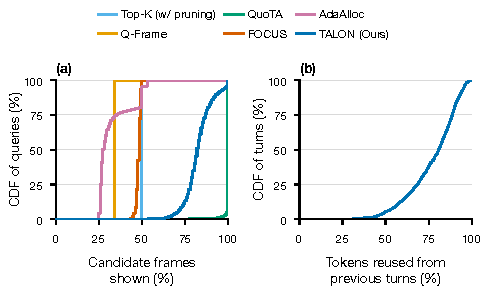
\includegraphics[width=\linewidth]{fig/overlap_pair.pdf}
  \caption{\textbf{What \name shows and reuses.} (a)~Share of the candidate frames that receive at least one token, per question. (b)~Share of the tokens that a turn needs which the KV cache already holds, for every turn after the first.}
  \label{fig:overlap}
\end{figure}

In a conversation, a user asks several questions $q_1,\dots,q_T$ about one video, and the KV cache of the conversation is kept between turns. Frame-level RAG fits this setting naturally: a later question appends only the frames it adds, and prefix caching reuses everything before them~\cite{kwon2023vllm,zheng2024sglang}. Token allocation, however, breaks this reuse, since solving Eq.~\eqref{eq:joint} afresh for each question changes the token counts of frames already in the context, even though consecutive questions share much of their evidence (\cref{fig:overlap}). \name instead carries the allocation across turns. At each turn $t$, it (1) updates the relevance of the cached frames with the attention of the VLM, (2) solves Eq.~\eqref{eq:joint} with the updated relevance, and (3) prefills only the tokens that the cache lacks.

\paragraph{Updating Relevance with Attention.}
Once a frame is cached, the VLM has already read it, and its attention to the frame indicates how much the frame matters for the new question. \name prefills $q_t$ on top of the cache, which the turn requires anyway, and measures the attention from the question tokens to the cached visual tokens in a few heads~\cite{rekv2025}. With $a_i$ the share of this attention per cached token of frame $f_i$, \name combines it with the retrieval relevance as
\begin{equation}
  r_i^{(t)}\propto r(f_i\mid q_t)^{1-\gamma}\,a_i^{\gamma}
  \label{eq:fusion}
\end{equation}
for cached frames, and keeps $r_i^{(t)}=r(f_i\mid q_t)$ for the others. Here, $\gamma\in[0,1]$ sets the trust in attention, from retrieval alone at $\gamma=0$ to attention alone at $\gamma=1$. We tune $\gamma$ to maximize the hypervolume of the accuracy--TFLOPs Pareto frontier, following standard multi-objective optimization~\cite{karl2023multiobjective,daulton2020qehvi}. The cached frames are then rescaled to keep their total relevance, so attention only re-ranks the frames the VLM has already seen and cannot take relevance from frames it has not seen.

\paragraph{Allocating and Prefilling.}
\name then solves Eq.~\eqref{eq:joint} with relevance $r_i^{(t)}$. Let $c_i$ be the tokens of frame $f_i$ already in the cache, with $c_i=0$ before the first turn. Rather than prefilling the new allocation $b_i$ in full, \name prefills only the $p_i=\max(0,b_i-c_i)$ tokens that the cache lacks and sets $c_i\leftarrow\max(c_i,b_i)$. Since the pruner ranks tokens independently of the query (\cref{sec:allocation}), the missing tokens are simply the ones ranked between $c_i+1$ and $b_i$. \name appends them after the conversation, since inserting them inside the block of their frame would invalidate every later cache entry. Because the RoPE of the VLM~\cite{bai2025qwen25vl} encodes the temporal and spatial position of each visual token, an appended token keeps its position within its frame, and only its place in the sequence changes. The budget $B$ thus still bounds the tokens that the VLM attends to, while only the prefill shrinks.

\paragraph{Bounded Prefill.}
\name designs its pruner to rank the tokens of each frame once, independently of the query, so that every turn only extends the nested token sequence of a frame, and each rank is prefilled at most once. The prefill of a conversation is therefore bounded, however many turns it lasts:

\begin{proposition}
\label{prop:bound}
Let $b_i^{(t)}$ and $p_i^{(t)}$ be the allocation and the prefill of frame $f_i$ at turn $t$. Then, for a conversation of any length $T$,
\begin{equation}
  \sum_{t=1}^{T}p_i^{(t)}=\max_t\,b_i^{(t)}\le b_{\max} .
\end{equation}
\end{proposition}

\noindent Proposition~\ref{prop:bound} shows that a conversation prefills at most the full tokens of the frames it ever shows, whereas re-allocating from scratch prefills $\sum_t\sum_ib_i^{(t)}$ tokens, which grows with every turn. Prior allocation methods, in contrast, select frames afresh for every question, so their prefill grows with the conversation. A detailed proof is provided in the appendix.

\section{Evaluation}
\label{sec:exp}

Unless
stated otherwise, every method draws from the same candidate frames, sampled from each video at 1 fps and kept at
their native resolution, and receives the same budget of 12,288 tokens per question. \name scores the relevance of each frame with SigLIP~2~\cite{siglip2} and of each transcript segment with
BGE~\cite{bge}, using the question together with its answer options as the query. \name fits $\tau$ on a validation split of each benchmark, which we create when the benchmark provides none, with videos disjoint from the evaluation videos, and keeps it fixed during evaluation. All hyperparameters ($\tau$, $\eta$, $\beta$, $\gamma$, $L$, and the softmax temperature) are tuned on these splits; their values and further implementation details are given in the appendix.

\subsection{Experimental Setup}
\label{sec:exp-setup}

\paragraph{Models.} Qwen3-VL-8B~\cite{bai2025qwen3vl}
encodes each frame at its native resolution, at one token per $32\times32$ pixels, whereas
InternVL3.5-4B~\cite{wang2025internvl35} encodes each $448\times448$ image tile into 256 visual tokens.

\paragraph{Benchmarks.} We use three long-video multiple-choice benchmarks. For MLVU~\cite{zhou2024mlvu}, we use the 2,174 questions of its development set. For LongVideoBench
(LVB)~\cite{wu2024longvideobench}, we use its validation set of 1,337 questions. Neither provides subtitles in our setting, so the input is visual only.
Video-MME~\cite{fu2024videomme} contains 2,700 questions on short, medium, and long videos; we use its subtitled
setting, in which subtitle tokens count toward the same budget. For the multi-turn setting, we use 200 conversations of
MT-Video-Bench (MTVB)~\cite{mtvideobench2025}, whose answers are scored by an LLM judge (Gemini~3.8 Flash); the judge prompt is given in the appendix.

\paragraph{Metrics.} We report accuracy together with compute, measured in TFLOPs per question: the prefill compute
of the language models of all VLMs that a method calls, summed over every call for that question. For conversations,
we sum the compute over all turns. Offline indexing is not counted. We focus on compute and cost rather than latency.

\paragraph{Baselines.} Uniform sampling is the plain VLM with uniformly sampled frames at the same budget. All other methods extend the same embedding-based RAG pipeline, and differ in how they turn its
candidates into the input of the VLM:
\begin{itemize}
  \item Top-K (w/ pruning): Retrieves the top-64 frames by relevance and keeps 192 tokens of each with the token
    pruner of \name. Its frame count is tuned on the validation splits (32 to 256 frames at the same budget), where accuracy varies by less than \simnum{1} point.
  \item Q-Frame~\cite{zhang2025qframe}: Shows frames at three resolutions by relevance rank. We replace its Long-CLIP scorer with SigLIP~2.
  \item QuoTA~\cite{luo2025quota}: Scores each frame with a small VLM after decoupling the question, and assigns
    each frame a number of tokens that grows with its score.
  \item FOCUS~\cite{zhu2026focus}: Selects keyframes from short clips by bandit exploration.
  \item AdaAlloc~\cite{an2026adaalloc}: Lets the VLM plan how to split the budget between sparse low-resolution
    frames and dense high-resolution frames (concurrent work).
\end{itemize}
Every baseline receives the same candidate frames and, on Video-MME, the same retrieved transcript segments, and each
reimplementation matches the published accuracy of its method in the original setting.
Graph-based RAG is also prevalent in video understanding systems~\cite{ren2025videorag,shen2025vgent,yan2025ava,yang2026g2frag,chen2026memdreamer,yan2026ecrag}. We therefore also pair \name with VideoRAG~\cite{ren2025videorag}, whose retrieved frames \name re-allocates under the same budget.

\subsection{Main Results}
\label{sec:exp-main}

\begin{table*}[t]
  \centering
  \small
  \renewcommand{\arraystretch}{1.08}
  \newcommand{\group}[1]{\rowcolor{groupbg}\multicolumn{10}{l}{\textit{#1}} \\}
  \newcommand{\maintab}{%
  \begin{tabular}{l cc cc ccccc}
    \toprule
    \multirow{2}{*}{Method} & \multicolumn{2}{c}{MLVU (w/o subtitles)} & \multicolumn{2}{c}{LVB (w/o subtitles)} & \multicolumn{5}{c}{Video-MME (w/ subtitles)} \\
    \cmidrule(lr){2-3} \cmidrule(lr){4-5} \cmidrule(lr){6-10}
    & Overall~$\uparrow$ & TFLOPs~$\downarrow$
      & Overall~$\uparrow$ & TFLOPs~$\downarrow$
      & Overall~$\uparrow$ & Short~$\uparrow$ & Medium~$\uparrow$ & Long~$\uparrow$
      & TFLOPs~$\downarrow$ \\
    \specialrule{\lightrulewidth}{\aboverulesep}{0pt}
    \group{Qwen3-VL-8B~\cite{bai2025qwen3vl}}
    Uniform sampling & \cellcolor{heat4}\simnum{72.8} & \cellcolor{heat1}\simnum{216} & \cellcolor{heat4}\simnum{61.9} & \cellcolor{heat1}\simnum{231} & \cellcolor{heat4}\simnum{71.2} & \cellcolor{heat3}\simnum{80.9} & \cellcolor{heat4}\simnum{70.8} & \simnum{61.9} & \cellcolor{heat1}\simnum{229} \\
    RAG                                                      & & & & & & & & & \\
    \quad + Top-K (w/ pruning) & \cellcolor{heat3}75.9 & \cellcolor{heat1}218 & \cellcolor{heat3}64.0 & \cellcolor{heat1}232 & \cellcolor{heat4}73.1 & \cellcolor{heat2}82.4 & \cellcolor{heat3}73.4 & 63.6 & \cellcolor{heat1}230 \\
    \quad + Q-Frame~\cite{zhang2025qframe}\venue{ICCV'25} & \cellcolor{heat3}74.7 & \cellcolor{heat1}209 & \cellcolor{heat2}65.7 & \cellcolor{heat1}225 & \cellcolor{heat4}71.1 & \cellcolor{heat3}80.1 & \cellcolor{heat4}70.3 & 63.0 & \cellcolor{heat0}218 \\
    \quad + QuoTA~\cite{luo2025quota}\venue{AAAI'26} & \cellcolor{heat2}77.2 & 781 & \cellcolor{heat1}66.6 & 676 & \cellcolor{heat3}74.4 & \cellcolor{heat1}83.2 & \cellcolor{heat3}74.4 & \cellcolor{heat4}65.4 & 647 \\
    \quad + FOCUS~\cite{zhu2026focus}\venue{ICLR'26} & \cellcolor{heat4}71.7 & \cellcolor{heat1}211 & \cellcolor{heat3}64.0 & \cellcolor{heat1}226 & \cellcolor{heat4}70.1 & \cellcolor{heat4}79.1 & \cellcolor{heat4}69.4 & 61.8 & \cellcolor{heat1}224 \\
    \quad + AdaAlloc~\cite{an2026adaalloc}\venue{NeurIPS'26} & \cellcolor{heat4}73.2 & \cellcolor{heat0}203 & \cellcolor{heat3}65.1 & \cellcolor{heat0}222 & \cellcolor{heat4}71.0 & \cellcolor{heat1}82.8 & \cellcolor{heat4}69.4 & 60.7 & \cellcolor{heat1}225 \\
    \quad + \textbf{\name (Ours)} & \cellcolor{heat1}78.1 & \cellcolor{heat2}230 & \cellcolor{heat1}66.6 & \cellcolor{heat1}234 & \cellcolor{heat1}77.3 & \cellcolor{heat0}\textbf{83.6} & \cellcolor{heat1}76.8 & \cellcolor{heat1}71.7 & \cellcolor{heat1}232 \\
    VideoRAG~\cite{ren2025videorag} & \cellcolor{heat3}\simnum{76.4} & \cellcolor{heat2}\simnum{226} & \cellcolor{heat3}\simnum{65.2} & \cellcolor{heat1}\simnum{238} & \cellcolor{heat3}\simnum{74.0} & \cellcolor{heat1}\simnum{82.6} & \cellcolor{heat3}\simnum{74.3} & \cellcolor{heat4}\simnum{65.1} & \cellcolor{heat1}\simnum{236} \\
    \quad + \textbf{\name (Ours)} & \cellcolor{heat0}\textbf{\simnum{78.6}} & \cellcolor{heat2}\simnum{233} & \cellcolor{heat0}\textbf{\simnum{67.3}} & \cellcolor{heat1}\simnum{239} & \cellcolor{heat0}\textbf{\simnum{77.6}} & \cellcolor{heat1}\simnum{83.4} & \cellcolor{heat0}\textbf{\simnum{77.1}} & \cellcolor{heat0}\textbf{\simnum{72.3}} & \cellcolor{heat1}\simnum{237} \\
    \specialrule{\lightrulewidth}{0pt}{0pt}
    \group{InternVL3.5-4B~\cite{wang2025internvl35}}
    Uniform sampling & \cellcolor{heat4}\simnum{69.8} & \cellcolor{heat1}\simnum{146} & \cellcolor{heat4}\simnum{58.6} & \cellcolor{heat1}\simnum{146} & \cellcolor{heat4}\simnum{65.6} & \cellcolor{heat3}\simnum{75.6} & \cellcolor{heat4}\simnum{65.3} & \simnum{55.9} & \cellcolor{heat1}\simnum{143} \\
    RAG                                                      & & & & & & & & & \\
    \quad + Top-K (w/ pruning) & \cellcolor{heat3}\simnum{72.5} & \cellcolor{heat1}\simnum{147} & \cellcolor{heat3}\simnum{60.4} & \cellcolor{heat1}\simnum{147} & \cellcolor{heat4}\simnum{67.7} & \cellcolor{heat2}\simnum{77.3} & \cellcolor{heat3}\simnum{68.1} & \simnum{57.8} & \cellcolor{heat1}\simnum{144} \\
    \quad + Q-Frame~\cite{zhang2025qframe}\venue{ICCV'25} & \cellcolor{heat3}\simnum{71.3} & \cellcolor{heat0}\simnum{141} & \cellcolor{heat2}\simnum{62.1} & \cellcolor{heat0}\simnum{142} & \cellcolor{heat4}\simnum{65.7} & \cellcolor{heat4}\simnum{75.0} & \cellcolor{heat4}\simnum{65.0} & \simnum{57.2} & \cellcolor{heat0}\simnum{136} \\
    \quad + QuoTA~\cite{luo2025quota}\venue{AAAI'26} & \cellcolor{heat3}71.3 & 708 & \cellcolor{heat2}62.5 & 583 & \cellcolor{heat4}64.9 & \cellcolor{heat4}74.7 & \cellcolor{heat4}64.6 & 55.4 & 551 \\
    \quad + FOCUS~\cite{zhu2026focus}\venue{ICLR'26} & \cellcolor{heat4}69.5 & \cellcolor{heat1}142 & \cellcolor{heat4}58.8 & \cellcolor{heat1}143 & \cellcolor{heat4}66.4 & \cellcolor{heat3}75.9 & \cellcolor{heat4}65.9 & 57.4 & \cellcolor{heat1}140 \\
    \quad + AdaAlloc~\cite{an2026adaalloc}\venue{NeurIPS'26} & \cellcolor{heat3}71.1 & 314 & \cellcolor{heat0}\textbf{63.6} & 331 & \cellcolor{heat4}67.9 & \cellcolor{heat0}\textbf{79.2} & \cellcolor{heat4}66.7 & 57.8 & 325 \\
    \quad + \textbf{\name (Ours)} & \cellcolor{heat0}\textbf{\simnum{74.7}} & \cellcolor{heat1}\simnum{155} & \cellcolor{heat1}\simnum{63.0} & \cellcolor{heat1}\simnum{148} & \cellcolor{heat0}\textbf{\simnum{72.0}} & \cellcolor{heat1}\simnum{78.5} & \cellcolor{heat0}\textbf{\simnum{71.5}} & \cellcolor{heat0}\textbf{\simnum{65.9}} & \cellcolor{heat1}\simnum{145} \\
    \specialrule{\heavyrulewidth}{0pt}{\belowbottomsep}
  \end{tabular}}%
  \sbox0{\setlength{\tabcolsep}{0pt}\maintab}%
  \setlength{\tabcolsep}{\dimexpr(\textwidth-\wd0)/20\relax}%
  \maintab
  \caption{\textbf{Main results.} Accuracy (\%) on MLVU, LongVideoBench (LVB), and Video-MME with subtitles at a
    budget of 12,288 tokens, with the compute (TFLOPs per question) of each method on each benchmark. Within each VLM
    block, darker cells are closer to the best value of their column, and the best accuracy is in bold.}
  \label{tab:main}
\end{table*}

\paragraph{\name achieves the Pareto frontier in single-turn question answering.}
\cref{tab:main} compares all methods at the budget of 12,288 tokens. With Qwen3-VL-8B and embedding-based RAG, \name
attains the highest accuracy on all three benchmarks, tied with QuoTA on LVB. At matched compute, it exceeds Q-Frame, FOCUS, and AdaAlloc by 0.9 to 7.2 points. Relative to Top-K (w/ pruning),
\name gains 2.2, 2.6, and 4.2 points on MLVU, LVB, and Video-MME. The gain is largest on the long videos of Video-MME (8.1 points), where the relevant evidence is sparse. QuoTA is the closest baseline: its difference to \name on MLVU and LVB is within one point and not significant (paired McNemar test, $p\ge0.12$),
but its per-frame scorer calls cost 2.8--3.4$\times$ more compute. The gains carry over to
InternVL3.5-4B: \name remains the most accurate method on MLVU and
Video-MME, where it improves on the best baseline by \simnum{2.2} and \simnum{4.1} points, and is within
\simnum{0.6} points of AdaAlloc on LVB at less than half of its compute. \name also transfers to graph-based retrieval: paired with VideoRAG, it gains
\simnum{2.2}, \simnum{2.1}, and \simnum{3.6} points on the three benchmarks at about the same compute.

\cref{fig:budget} and \cref{fig:multiturn}(a) vary the budget from 1,536 to 12,288 tokens on MLVU. \name is the most
accurate method at every budget, and its advantage grows as the budget shrinks: at 1,536 tokens it reaches 73.4\%, 8.3 points above Top-K (w/ pruning). With 3,072 tokens (53 TFLOPs), it exceeds the accuracy of Q-Frame,
FOCUS, and AdaAlloc at 12,288 tokens (203--211 TFLOPs), a reduction of nearly 4$\times$.

\begin{figure}[t]
  \centering
  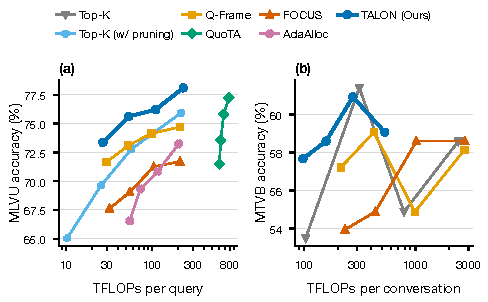
\includegraphics[width=\linewidth]{fig/tflops_pair.pdf}
  \caption{\textbf{Accuracy against compute.} (a)~Single turn: MLVU accuracy against TFLOPs per query.
    (b)~Multi turn: MT-Video-Bench accuracy (a 100-conversation subset for the four-budget sweep, 215 judged turns) against TFLOPs per conversation, summed over all turns. Each line spans per-turn budgets from 1,536 to 12,288 tokens.}
  \label{fig:multiturn}
\end{figure}

\paragraph{\name achieves the Pareto frontier across multi-turn conversations.}
\cref{fig:multiturn}(b) reports accuracy against the compute of a whole conversation on MT-Video-Bench. All methods keep the KV cache across turns, and a baseline skips a frame that the cache already holds at the selected
resolution. The baselines still add the new frames of every question, whereas \name prefills only the tokens that the
cache lacks. At the same
per-turn budget, it consequently uses 2.2--5.2$\times$ less compute than Q-Frame and FOCUS and up to 4.6$\times$ less
than Top-K (w/ pruning), and it is the most accurate method at three of the four budgets. A turn after the first finds a median of 81\% of its tokens already in the cache
(\cref{fig:overlap}(b)).

\begin{table}[t]
  \centering
  \small
  \renewcommand{\arraystretch}{1.2}
  \settowidth{\splitw}{Medium}%
  \newcommand{\abltab}{%
  \begin{tabular}{l@{\hspace{5pt}} c VVVV}
    \toprule
    Method & TFLOPs $\downarrow$
      & \multicolumn{4}{c}{%
        \begin{tabular}{@{}VVVV@{}}
          \multicolumn{4}{c}{Video-MME (w/ subtitles) $\uparrow$} \\
          \cmidrule(lr){1-4}
          Overall & Short & Medium & Long \\[2.6pt]
        \end{tabular}} \\
    \specialrule{\lightrulewidth}{\aboverulesep}{0pt}
    \textbf{\name} & \cellcolor{heat1}232 & \cellcolor{heat0}\textbf{77.3} & \cellcolor{heat0}\textbf{83.6} & \cellcolor{heat0}\textbf{76.8} & \cellcolor{heat0}\textbf{71.7} \\
    \hspace{0.5em}w/o water-filling & \cellcolor{heat1}\simnum{229} & \cellcolor{heat3}\simnum{74.8} & \cellcolor{heat1}\simnum{83.4} & \cellcolor{heat1}\simnum{76.0} & \cellcolor{heat4}\simnum{64.9} \\
    \hspace{0.5em}w/o text allocation & \cellcolor{heat0}226 & \cellcolor{heat3}73.7 & \cellcolor{heat2}81.9 & \cellcolor{heat2}74.9 & \cellcolor{heat4}64.4 \\
    \hspace{0.5em}w/o diversity & \cellcolor{heat0}226 & \cellcolor{heat1}76.6 & \cellcolor{heat2}82.4 & \cellcolor{heat1}76.4 & \cellcolor{heat1}70.8 \\
    \bottomrule
  \end{tabular}}%
  \sbox0{\setlength{\tabcolsep}{0pt}\abltab}%
  \setlength{\tabcolsep}{\dimexpr(\columnwidth-\wd0)/11\relax}%
  \xdef\ablsep{\the\tabcolsep}%
  \abltab
  \caption{\textbf{Ablation of the Token Scheduler} on Video-MME with subtitles (Qwen3-VL-8B, 12,288 tokens). Each
    row removes one component of \name.}
  \label{tab:ablation}
\end{table}

\paragraph{Performance breakdown.}
\cref{tab:ablation} removes one component of the Token Scheduler at a time. Replacing water-filling with an
allocation proportional to relevance, at matched compute, lowers accuracy by \simnum{2.5} points overall and by
\simnum{6.8} points on long videos. Removing text allocation, so that each shown frame only brings its time-aligned subtitles, costs 3.6 points overall and 7.3 points on long videos. Removing the
diversity term costs 0.7 points. The vision encoder runs once per video, at 48 TFLOPs, and its output is reused across questions and turns.

\cref{tab:multiturn} ablates the two multi-turn components at 6,144 tokens per turn. Updating relevance with the
attention of the VLM improves accuracy by 1.1 points and reduces compute by 13\%, since attention concentrates the
allocation on frames that the cache already holds. Without the carried allocation, every turn recomputes its evidence
from scratch, which raises compute by \simnum{2.3}$\times$ with no gain in accuracy; appending tokens thus costs no accuracy. A sensitivity analysis of the
hyperparameters is given in the appendix.

\begin{table}[t]
  \centering
  \small
  \renewcommand{\arraystretch}{1.2}
  \setlength{\tabcolsep}{\ablsep}%
  \settowidth{\dimen0}{\hspace{0.5em}w/o carried allocation}%
  \dimen2=\dimexpr(\columnwidth-5\tabcolsep-5pt-\dimen0)/2\relax
  \begin{tabular}{l@{\hspace{5pt}} >{\centering\arraybackslash}p{\dimen2} >{\centering\arraybackslash}p{\dimen2}}
    \toprule
    Method & TFLOPs $\downarrow$ & MTVB (w/o subtitles) $\uparrow$ \\
    \midrule
    \textbf{\name} & \cellcolor{heat0}275 & \cellcolor{heat0}\textbf{58.5} \\
    \hspace{0.5em}w/o attention & \cellcolor{heat2}315 & \cellcolor{heat2}57.4 \\
    \hspace{0.5em}w/o carried allocation & \simnum{640} & \cellcolor{heat1}\simnum{58.2} \\
    \bottomrule
  \end{tabular}
  \caption{\textbf{Ablation of multi-turn scheduling} on MT-Video-Bench (Qwen3-VL-8B; 200 conversations, 450 judged turns; 6{,}144
    visual tokens per turn). TFLOPs are summed over all turns of a conversation.}
  \label{tab:multiturn}
\end{table}

\section{Conclusion}
\label{sec:conclusion}

\paragraph{Limitations and future work.}
\name allocates tokens according to the relevance scores of the retriever, and cannot recover evidence that the
retriever scores as irrelevant. Moreover, all frames share one token value function, although a frame with dense on-screen text
likely saturates later; predicting it per frame is a natural extension. Finally, our multi-turn evaluation covers one VLM.

\paragraph{Conclusion.}
We presented \name, which moves video RAG from selecting frames to allocating tokens, within a turn and across the
turns of a conversation. Across three benchmarks and two VLMs, it improves accuracy at equal compute and matches the
strongest prior method at roughly one third of its compute.
\par

\else
\begin{abstract}
Retrieval-augmented generation (RAG) allows video large language models (VLMs) to answer questions about hours of
footage by showing them only the frames most relevant to a query. Existing VideoRAG systems, however, decide only which
frames to show, and encode every retrieved frame with the same number of tokens. We introduce \name, a plug-and-play
framework that lifts video RAG from the frame level to the token level. Rather than keeping the $K$ most relevant
frames at a fixed cost, \name models the value of a frame as its relevance weighted by a measured token--quality
curve, and allocates one token budget across frames and transcript text by solving a sparse integer program exactly
with a single token price. For multi-turn conversations, \name further introduces multi-turn allocation, which reuses
the KV cache across questions through a rank-only pruner, so that each turn prefills only the tokens the cache does
not yet hold and the total prefill of every frame is bounded by its largest allocation. On LVBench with
Qwen2.5-VL-7B, \name improves accuracy over top-$K$ frame retrieval at every matched budget, from 45.4\% to 54.6\% at
9.6k tokens and from 54.6\% to 62.9\% at 76.5k tokens. On MT-Video-Bench, multi-turn allocation reduces visual
prefill by 2.2$\times$ relative to re-prefilling every turn, with no significant change in score.
\end{abstract}
    
\section{Introduction}
\label{sec:intro}

\begin{figure}[t]
  \centering
  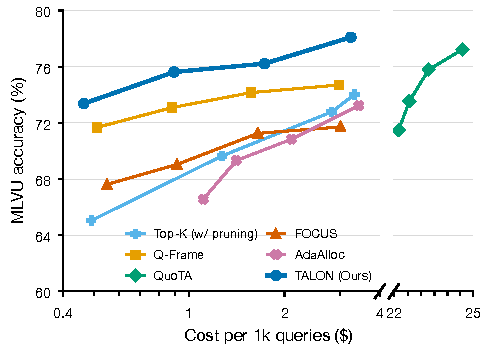
\includegraphics[width=\linewidth]{fig/budget_curve.pdf}
  \caption{\TODO{}}
  \label{fig:budget}
\end{figure}

\fyy{It turns out token compression is a popular method for video understanding (e.g., \href{https://arxiv.org/pdf/2510.07915}{retrieve-then-compress} and \href{https://arxiv.org/abs/2410.17434}{adaptive compression}). See my Teams message.}

\fyy{Therefore, a safer and better title and narrative should be
something like ``Efficient Video RAG through Token Allocation''.
Our keywords are token efficiency and token allocation (in a globally optimal manner, rather than greedy, independent compression).}

\fyy{My current thinking for the intro outline is as follows
(each point is a paragraph):
\begin{enumerate}
\item \textit{Problem \& importance.}
Briefly introduce VLM-based video understanding, then quickly
move to our problem setting of \textit{long} video understanding.
Establish its importance through concrete application domains.
\item \textit{RAG is commonly used for long video understanding.}
Processing all tokens from long videos can easily
exceed VLM context windows and incur high compute costs.
Therefore, existing systems widely resort to
RAG, notably embedding-based and graph-based approaches,
to supply relevant
visual or textual evidence for each query.
\item \textit{Limitations of existing approaches.}
Graph-based RAG achieves high benchmark accuracy,
but video ingestion is expensive and often wasted
since users tend to ask questions sporadically.
Embedding-based RAG is more lightweight, but our motivating
experiments in Section 2 reveal its limitations.
Adding tokens to a relevant frame yields diminishing returns.
Although video token compression mitigates this issue,
independently compressing retrieved frames
is also suboptimal,
as a different allocation of the global token budget
could reveal useful evidence in other frames.
\item \textit{Our insight and method.}
These limitations motivate us to jointly allocate
tokens across frames according to their contribution
to answering the query.
We present \name, a token-efficient video RAG framework
that preserves QA accuracy.
\name formulates video RAG as a token allocation problem
under a limited budget.
\item \textit{Challenges faced by \name and our solutions.}
Challenge 1 / solution 1 centers on
offline profiling of token value
and exact token allocation.
Challenge 2 / solution 2 is multi-turn conversations.
\item \textit{Evaluation highlights.}
\item \textit{Contributions and three bullet points.}
\end{enumerate}
}

paragraph 1: introduce video understanding

paragraph 2: highlight the problem of long context video understanding, introduce RAG methods for video understanding

paragraph 3: prior work is frame level, admits every frame at equal cost, however, relevant frames vary in relevance point to Fig X (x axis: frames, y axis relevance score). motivate token level design.

paragraph 4: highlight unique challenges,  characteristics we want from a strong design. 

paragraph 5: We introduce a plug-and-play \textbf{T}oken \textbf{AL}locati\textbf{ON} (\name) framework. quick pass through the framework, should demonstrate points in paragraph 4 are addressed.

% Our contributions are as follows:
% \begin{itemize}
%   \item We introduce \name, a plug-and-play framework that moves existing VideoRAG systems from frame-level RAG to token-level RAG.
%   \item We design a low-cost token scheduling algorithm from a principled optimization perspective, which jointly allocates tokens across frames and transcripts, using each modality for what it does best, and composes the resulting evidence into a temporally ordered storyboard. It improves on prior keyframe selection and token allocation methods both theoretically and empirically.
%   \item We extend token scheduling to multi-turn conversations, where the attention of the VLM updates the allocation of frames it has already seen, and new tokens are appended to the KV cache so that the total prefill stays bounded however long the conversation lasts.
%\end{itemize}
Across multiple VideoRAG backbones, \name achieves \todo{[TODO: A--B]}$\times$ higher accuracy than conventional frame retrieval and prior keyframe selection methods at matched compute budgets.



\section{Related Work}
\label{sec:related}

\paragraph{Video retrieval augmented generation.}
RAG grounds generation in retrieved evidence. For long videos, Video-RAG~\cite{luo2024videorag} augments a VLM with
visually aligned auxiliary texts, such as speech transcripts, on-screen text, and detected objects, retrieved for each
query. VideoRAG~\cite{ren2025videorag} instead builds a graph-based knowledge index across videos, and
Vgent~\cite{shen2025vgent} represents a video as a graph of clips that preserves their semantic and temporal
dependencies, followed by a structured reasoning step that filters retrieval noise. These systems, however, focus on
what to index and retrieve, and pass every retrieved item to the VLM at its full cost. \name instead decides how many
tokens each retrieved item receives, and can be placed after any of these retrievers. \ayush{add more cites, maybe ~6 more, mention AVA}

\paragraph{Keyframe selection.}
Most VLMs sample frames uniformly and therefore often miss the content that a query needs. Query-aware methods instead
select frames by jointly optimizing their relevance and temporal coverage~\cite{tang2025aks,peng2026qca}, by greedy
marginal utility~\cite{shi2026markey}, by learning to query informative combinations of
frames~\cite{yu2024framevoyager}, or with the attention of a small VLM used as a selector~\cite{wang2026dafs}. All of
these methods, however, return a subset of frames, each at the same token cost. \name instead treats the token count
of each frame as a decision variable.


\section{Method}
\label{sec:method}

\begin{figure*}[t]
  \centering
  \makebox[\linewidth][c]{% Overview figure (figure*, drawn at \textwidth = 17.46 cm). The Overleaf figure (fig/overview_v1.tex), refined:
% numbered stages with a one-line description each, single-turn inference only (no KV cache), less empty space,
% larger frames and text. Three stages left to right:
% (1) retrieval: video + subtitles -> retriever (with query q) -> relevance r_i over items in time order;
% (2) Token Scheduler (the contribution, the only accented stage): objective, value curves v_frame / v_text,
%     water-filling -> token plan b_i;
% (3) inference: frozen pruner keeps each frame's top-ranked tokens, the frozen VLM answers.
% Bar heights and the plan are illustrative, not measured. Frames: Video-MME video bepwr1-CNRU (illustration only).
% Tableau 10 (Stone, 2016): blue 4E79A7 and orange F28E2B on neutral greys; dark text on light fills only
\definecolor{ink}{HTML}{333333}%
\definecolor{arrowgray}{HTML}{6F6F6F}%
\definecolor{bandA}{HTML}{F4F5F7}%
\definecolor{bandB}{HTML}{EAF1F8}%
\definecolor{edgeB}{HTML}{4E79A7}%
\definecolor{bandC}{HTML}{F4F5F7}%
\definecolor{stepA}{HTML}{333333}%
\definecolor{stepB}{HTML}{4E79A7}%
\definecolor{stepC}{HTML}{333333}%
\definecolor{modelA}{HTML}{DCE6F1}%
\definecolor{modelC}{HTML}{DCE6F1}%
\definecolor{modelD}{HTML}{4E79A7}%
\definecolor{modelT}{HTML}{333333}%
\definecolor{flake}{HTML}{4E79A7}%
\definecolor{chipF}{HTML}{FFFFFF}%
\definecolor{chipD}{HTML}{A0A0A0}%
\definecolor{frm}{HTML}{4E79A7}%
\definecolor{txt}{HTML}{F28E2B}%
\definecolor{accA}{HTML}{4E79A7}%
% every color role: ink, arrowgray, bandA/B/C, edgeB, stepA/B/C, modelA/C/D/T, flake, chipF/D, frm, txt
\newcommand{\snowflake}[2]{%
  \begin{scope}[shift={#1}, line width=0.55pt, draw=flake, line cap=round]
    \foreach \a in {0,60,...,300}{\draw (0,0) -- (\a:#2);
      \draw (\a:0.55*#2) -- ++(\a+45:0.32*#2); \draw (\a:0.55*#2) -- ++(\a-45:0.32*#2);}
  \end{scope}}
% \items{width}{height scale}{v1/t1,...,v20/t20}: 20 items on one time axis; t = 1 marks a transcript event (light bar)
\newcommand{\items}[3]{%
  \foreach \v/\t [count=\i] in {#3} {
    \ifnum\t=1 \fill[txt] ({(\i-0.5)*#1/20-0.3*#1/20},0) rectangle ++({0.6*#1/20},{\v*#2});
    \else      \fill[frm]    ({(\i-0.5)*#1/20-0.3*#1/20},0) rectangle ++({0.6*#1/20},{\v*#2}); \fi}}
% \prunedframe{center}{image}{kept tokens out of 32}: a frame (1.0 cm) as an 8x4 token grid; dropped tokens greyed out.
% The keep order is one fixed ranking (centre first), so a frame at b tokens holds its top b tokens.
\newcommand{\prunedframe}[3]{%
  \node[inner sep=0pt] at (#1) {\includegraphics[width=1.0cm]{fig/frames/#2}};
  \begin{scope}[shift={($(#1)+(-0.5,-0.28125)$)}]
    \foreach \c [count=\k from 0] in {10,11,18,19,9,12,17,20,2,3,26,27,1,4,25,28,8,13,16,21,0,5,24,29,6,14,22,30,7,15,23,31} {
      \ifnum\k<#3\relax\else
        \pgfmathtruncatemacro{\cx}{mod(\c,8)}\pgfmathtruncatemacro{\cy}{int(\c/8)}
        \fill[white, opacity=0.85] (\cx*0.125,\cy*0.140625) rectangle ++(0.125,0.140625);
      \fi}
    \draw[ink!30, line width=0.15pt, xstep=0.125, ystep=0.140625] (0,0) grid (1.0,0.5625);
    \draw[ink!45, line width=0.3pt] (0,0) rectangle (1.0,0.5625);
  \end{scope}}
\newcommand{\txtchip}[1]{% transcript event: a short text chip
  \fill[txt!35, rounded corners=1pt] ($(#1)+(-0.42,-0.2)$) rectangle ++(0.84,0.4);
  \draw[txt!85!black, line width=0.5pt] ($(#1)+(-0.3,0.07)$) -- ++(0.6,0);
  \draw[txt!85!black, line width=0.5pt] ($(#1)+(-0.3,-0.07)$) -- ++(0.4,0);}
% \stage{x}{y}{number}{title}{one-line description}: numbered stage heading
\newcommand{\stage}[5]{%
  \node[circle, fill=#5, text=white, font=\sffamily\scriptsize\bfseries, inner sep=0pt, minimum size=0.4cm] at (#1+0.2,#2) {#3};
  \node[font=\sffamily\small\bfseries, text=#5, anchor=west, inner sep=0pt] at (#1+0.5,#2) {#4};}

\begin{tikzpicture}[font=\sffamily\footnotesize, text=ink, line width=0.6pt,
  card/.style={fill=white, draw=ink!18, line width=0.5pt, rounded corners=4pt, align=center, inner sep=3.5pt},
  arr/.style={-{Stealth[length=5pt, width=4pt]}, draw=arrowgray, line width=0.8pt},
  ax/.style={-{Stealth[length=3.5pt, width=3pt]}, draw=ink!55, line width=0.5pt},
  axl/.style={font=\sffamily\scriptsize, text=ink!70},
  desc/.style={font=\sffamily\scriptsize, text=ink!65, anchor=north west, inner sep=0pt, align=left},
  elbl/.style={font=\sffamily\scriptsize, text=ink!75, inner sep=1.5pt},
  model/.style={fill=modelC, draw=modelD, text=modelT, line width=0.5pt, rounded corners=3pt, align=center,
    minimum height=0.62cm, inner xsep=5pt, font=\sffamily\footnotesize},
  qa/.style={fill=chipF, draw=chipD, line width=0.5pt, rounded corners=3pt, align=left,
    inner sep=3pt, font=\sffamily\scriptsize}]

% ---------------- layout ----------------
% Top row: (1) Retrieval -> (2) Allocation; bottom row: (3) Inference, left to right. Stages connect box to box
% (r_i, b_i). Q sits inside Retrieval and A inside Inference; nothing is outside the stage boxes.
\fill[rounded corners=6pt, bandA] (0,2.0) rectangle (7.5,5.3);
\fill[rounded corners=6pt, bandB] (8.0,2.0) rectangle (17.4,5.3);
\draw[rounded corners=6pt, edgeB, line width=0.6pt] (8.0,2.0) rectangle (17.4,5.3);
\fill[rounded corners=6pt, bandC] (0,0) rectangle (17.4,1.6);
\stage{0.12}{5.02}{1}{Retrieval}{stepA}
\stage{8.12}{5.02}{2}{Allocation}{stepB}
\stage{0.12}{1.3}{3}{Inference}{stepC}
\draw[arr] (7.5,3.65) -- node[elbl, above] {$r_i$} (8.0,3.65);
\draw[arr] (12.7,2.0) -- node[elbl, right] {$b_i$} (12.7,1.6);

% ---------------- (1) retrieval ----------------
\fill[ink!88, rounded corners=1pt] (0.2,3.85) rectangle (7.3,4.75);
\foreach \x in {0.28,0.48,...,7.2} {\fill[white] (\x,4.65) rectangle ++(0.1,0.06); \fill[white] (\x,3.89) rectangle ++(0.1,0.06);}
\foreach \k in {1,...,5} {\node[inner sep=0pt] at ({0.91+(\k-1)*1.42},4.3) {\includegraphics[width=1.2cm]{fig/frames/frame\k.jpg}};}
\fill[txt!35, rounded corners=1pt] (0.2,3.57) rectangle (7.3,3.77);
\foreach \x/\l in {0.5/1.0, 1.9/0.8, 3.1/1.2, 4.7/0.9, 6.0/0.9} {\draw[txt!85!black, line width=0.5pt] (\x,3.67) -- ++(\l,0);}
\node[qa] (q) at (1.0,2.75) {\textbf{Q:} Color of\\the last car?};
\node[model, fill=modelA] (ret) at (2.95,2.75) {Retriever\hspace{0.12cm}};
\snowflake{($(ret.north east)+(-0.14,-0.14)$)}{0.075}
\draw[arr] (q.east) -- (ret.west);
\draw[arr] (2.95,3.55) -- (ret.north);
\begin{scope}[shift={(4.25,2.42)}]
  \draw[ax] (0,0) -- (3.05,0); \draw[ax] (0,0) -- (0,1.0);
  \node[axl, anchor=west] at (0.06,0.93) {$r_i$};
  \node[axl, anchor=north] at (1.5,-0.02) {frame \#};
  \items{2.95}{1.4}{.04/0,.06/0,.30/0,.52/0,.20/1,.40/0,.10/0,.05/0,.04/0,.36/1,
                   .06/0,.22/0,.30/0,.42/1,.34/0,.26/0,.08/0,.18/1,.05/0,.03/0}
\end{scope}
\draw[arr] (ret.east) -- (4.15,2.75);

% ---------------- (2) allocation ----------------
\node[font=\sffamily\scriptsize] at (12.7,4.5) {$\max\limits_{\mathbf b}\ \sum_i r_iv_i(b_i)-\eta\sum_{i\neq j}s_{ij}\,v_i(b_i)\,v_j(b_j)\qquad\text{s.t.}\ \ \sum_i b_i\le B$};
\begin{scope}[shift={(8.75,2.42)}]
  \draw[ax] (0,0) -- (3.2,0); \draw[ax] (0,0) -- (0,1.6);
  \node[axl, anchor=west] at (0.06,1.5) {$v(b)$};
  \node[axl, anchor=north] at (1.6,-0.02) {$b$};
  \draw[txt, line width=1.1pt, domain=0.02:8, samples=60] plot ({0.37*\x}, {1.45*((2^\x-1)^0.841)/(((2^\x-1)^0.841)+3.44)});
  \draw[frm, line width=1.1pt, domain=0.02:8, samples=60] plot ({0.37*\x}, {1.35*((2^\x-1)^0.841)/(((2^\x-1)^0.841)+7.73)});
  \node[font=\sffamily\scriptsize, text=txt!80!black, anchor=south west, inner sep=1pt] at (3.0,1.35) {$v_{\text{text}}$};
  \node[font=\sffamily\scriptsize, text=frm, anchor=north west, inner sep=1pt] at (3.0,1.2) {$v_{\text{frame}}$};
\end{scope}
\draw[arr] (12.75,3.2) -- (13.45,3.2);
\begin{scope}[shift={(13.85,2.42)}]
  \draw[ax] (0,0) -- (3.3,0); \draw[ax] (0,0) -- (0,1.6);
  \node[axl, anchor=west] at (0.06,1.5) {$b_i$};
  \node[axl, anchor=north] at (1.6,-0.02) {frame \#};
  \items{3.2}{1.9}{0/0,0/0,.438/0,.688/0,.25/1,.531/0,0/0,0/0,0/0,.5/1,
                   0/0,.25/0,.344/0,.5/1,.406/0,.312/0,0/0,.25/1,0/0,0/0}
\end{scope}

% ---------------- (3) inference ----------------
% the frozen pruner is a container that holds its output: the frames at their token counts and the text events
\node[model, minimum width=9.4cm, minimum height=1.0cm] (pr) at (7.3,0.7) {};
\node[font=\sffamily\footnotesize, text=modelT, align=center] at (3.4,0.7) {Token\\pruner};
\snowflake{($(pr.north east)+(-0.14,-0.14)$)}{0.075}
\prunedframe{4.95,0.7}{frame1.jpg}{6}
\txtchip{6.15,0.7}
\prunedframe{7.35,0.7}{frame3.jpg}{22}
\prunedframe{8.55,0.7}{frame4.jpg}{12}
\txtchip{9.75,0.7}
\prunedframe{10.95,0.7}{frame5.jpg}{32}
\node[model, minimum width=2.4cm, minimum height=1.0cm] (vlm) at (14.0,0.7) {VLM};
\snowflake{($(vlm.north east)+(-0.14,-0.14)$)}{0.075}
\node[qa] (ans) at (16.4,0.7) {\textbf{A:} Blue};
\draw[arr] (pr.east) -- (vlm.west);
\draw[arr] (vlm.east) -- (ans.west);
\end{tikzpicture}
}
  \caption{\textbf{\name overview.} \ayush{overview description. make the figure ore beautiful.}}
  \label{fig:overview}
\end{figure*}

% ---------------------------------------------------------------------------------------------------------------------
\subsection{Overview and Problem Formulation}
\label{sec:overview}

Frame-level RAG answers a user query $q$ about a video $V$ by passing the top-$K$ most semantically relevant frames to a VLM~\cite{}. Let $f_1, \dots, f_N$ be frames sampled uniformly from $V$, and let $r(f_i\mid q)$ denote the semantic similarity of $f_i$ with respect to $q$ (e.g., CLIP score~\cite{}), normalized across all frames, so that $r(\cdot\mid q)$ approximates the probability that each frame holds the evidence for $q$. Viewed from a mathematical angle, our frame allocation decision is a binary admit or reject, subject to a budget of $K$ frames, so as to maximize the total similarity of the admitted frames. Frame-level RAG is therefore naturally modeled as an integer linear program:
\begin{equation}
  \max_{\mathbf{x} \in \{0,1\}^N} \sum_{i=1}^{N} r(f_i\mid q)\, x_i \qquad \text{s.t.} \quad \sum_{i=1}^{N} x_i \le K.
  \label{eq:topk}
\end{equation}
where $f_i$ is passed to the VLM if $x_i=1$ and dropped if $x_i=0$. We lift this frame-level objective to a multimodal token-level objective, which carefully defines \textit{how} tokens should be scored, and prove that our solution is theoretically more optimal for this objective compared to naive adaptive token allocation baselines (\cref{sec:allocation}). In multi-turn conversations, however, naively re-allocating tokens at every turn is inefficient and breaks prefix caching~\cite{}, a standard feature of serving pipelines. We therefore reformulate our optimization objective to reuse the KV cache across turns. This improves both efficiency and accuracy, and we prove that the cumulative prefill cost stays bounded over long conversations due to our token pruner design (\cref{sec:multiturn}).


% ---------------------------------------------------------------------------------------------------------------------
\subsection{Token Allocation}
\label{sec:allocation}

Moving to token level RAG replaces the binary decision $x_i$ by $b_i$, where $b_i$ represents the number of tokens allocated to frame $f_i$, and the frame budget $K$ by a token budget $B$. Doing so, however, poses two key challenges. First, the objective must state what a frame is worth at every token count. Second, near-duplicate frames that repeat the content of others may be selected, so the relevance of a frame must account for already selected frames (inaccurate? as its account for frames weighted by the tokens allocated to them?). \name addresses the first challenge with a token value function calibrated offline (you can calibrated offline and continously calibrated across examples, then now R can be "updated" which you can define in a simple way), and the second by conditioning relevance on the allocation. We formulate both for frames alone and then extend the formulation to the transcript of the video. (not well written)

\paragraph{Measuring Token Value.}
Intuitively, the token count of a frame acts as its effective resolution. With few tokens, the VLM perceives only the coarse structure of the frame, such as the scene layout and large objects; with more tokens, it also perceives fine detail, such as small objects and on-screen text. How this added detail translates into downstream accuracy, however, is not known in advance, yet it decides how many tokens a frame deserves. We capture it with a \textit{token value function} $v(b)$, the probability (prefer not to say probability as reviewers may get angry) that the VLM reads the evidence of a frame shown with $b$ tokens, and lift~\eqref{eq:topk} to (did not mention how we got v, e.g. we took N video query pairs blah blah)
\begin{equation}
  \max_{\mathbf b}\ \sum_{i}r(f_i\mid q)\,v(b_i)\qquad\text{s.t.}\quad\sum_{i}b_i\le B .
  \label{eq:relevance}
\end{equation}
The objective is thus the probability that the evidence is both in the prompt and readable (dont say probability as its not really literal probability). Maximizing it is the (maybe put "Fig. Y" somewhere thsi is the figure for this offline curve ill add later)
classical problem of optimal search~\cite{koopman1956,stone1975}, with relevance as the prior over the location of the
evidence and tokens as the search effort. Top-$K$ retrieval~\eqref{eq:topk} is the special case $b_i\in\{0,b_{\max}\}$
and $B=Kb_{\max}$, where $b_{\max}$ is the token count of a full frame.

The objective is only as good as its value function. A linear $v$ would reward every token equally and ignore that a
frame saturates, whereas a step at a fixed count would reproduce the all-or-nothing cost of~\eqref{eq:topk}. \name
instead measures $v$ once per VLM, offline. Across a set of calibration videos and queries, it uniformly varies the
number of tokens per frame and fits
\begin{equation} (hmm i change my mind should mention value function FIRST then the objective function)
  v(b)=\frac{b^{\alpha}}{b^{\alpha}+\tau^{\alpha}}
  \label{eq:curve}
\end{equation}
to the probability that the VLM assigns to the correct answer, where $\tau$ is the token count at which a frame reaches
half of its value and $\alpha$ sets how sharply the value rises. (do not say per VLM, just stick to it. We measure V offline, then later sort of and it is updated online and we can sort of define that. Yeah, and kind of fix up the writing, make it write better. No need to say top K retrieval is a special case.

It's kind of obvious. Also never, never say this. Top K retrieval bracket one. That's not how you refer to things.

You say equation. Equation one, equation two. You don't just say brackets one. Hope people know what that means. No one knows what that means.

Maximizing two alone. No, you don't say maximizing equation 2. What is 2? Is it an equation? Is it a function? What is it? Never say stuff like this.

Also, no need to say top K retrieval. No need to mention classical problem of optimal search again stick to the topic measuring token value right we're giving intuition and we're essentially wanting to say okay well that's the intuition uh we need this and we measure this by this offline curve.

Okay, and this is the function. It's updated online. Make and you're putting this into objective function. Objective function looks like this. So there, I explained what v is.

I showed you the equation for v offline as well as online and then I showed you what the objective function is. And done, that's literally it. There's nothing else. Yeah. Very straightforward. Right? No need to mention all this optimal search. What is the relevance to that?

There is no relevance as a prior over the location of no, there is no prior, there is no location. Stop adopting this Bayesian framework. There is nothing Bayesian about. There is no prior.

There is no probabilities here like it's we use probability once like uh try to avoid that term because that's very inaccurate like the reviewer will be angry at you so again so see how I explain very logically follows very logically so that's the measuring token value)

\paragraph{Incorporating Frame Diversity.}
Maximizing~\eqref{eq:relevance} alone, however, spreads the budget too thin. Because the measured curve has $\alpha<1$,
its slope is unbounded at zero tokens, so the optimum gives tokens to every frame with nonzero relevance. Most of these
frames add little, since consecutive frames often show the same content, yet $v$ is measured one frame at a time and
credits every copy in full. Each additional frame is also a potential distractor for the VLM. The root cause is that
$r(f_i\mid q)$ depends on the query alone, whereas a frame tells the VLM little once a similar frame is already shown in
detail. We, therefore, condition the relevance of a frame on the allocation as well:
\begin{equation}
  r(f_i\mid q,\mathbf b)=r(f_i\mid q)-\eta\sum_{j\neq i}s_{ij}\,v(b_j) ,
  \label{eq:cond}
\end{equation}
where $s_{ij}$ measures whether $f_i$ and $f_j$ show the same content and $\eta$ sets how strongly the coverage by
similar frames discounts relevance. Pixel differences are poorly suited for $s_{ij}$, since camera motion changes pixels
without changing content. Temporal distance is also insufficient, since a scene can return much later in the video. We,
therefore, use the cosine $s_{ij}=\max\big(0,\cos(f_i,f_j)\big)$ of the image embeddings that the retriever already
computes. With the conditioned relevance, \name solves
\begin{equation}
  \max_{\mathbf b}\ \sum_{i}r(f_i\mid q,\mathbf b)\,v(b_i)\qquad\text{s.t.}\quad\sum_{i}b_i\le B .
% Ordered pairs (j != i) as in cover_allocate.py, so this eta equals the code's beta.
  \label{eq:p1}
\end{equation}
The objective keeps the form of~\eqref{eq:relevance}, and only the relevance changes. A frame thus loses relevance only
when similar frames are shown with many tokens, so the plan prefers frames with different content. Moreover, a frame
whose conditioned relevance falls to zero receives no tokens at all, so redundancy limits how many frames are shown
without a separate price per frame. A larger $\eta$ yields fewer, more distinct frames, while $\eta=0$
recovers~\eqref{eq:relevance}.

\paragraph{Extending to Transcripts.}
Many questions hinge on what is said rather than shown, so \name also allocates tokens to the transcript of the video.
The extension adds terms of the same form rather than a new mechanism. Let $u_1,\dots,u_M$ be the transcript events,
and index frames and events jointly as items $i\in[N+M]$, with $b_i$ the tokens of item $i$. We abbreviate the query
relevance of item $i$ as $r_i$, which is $r(f_i\mid q)$ for a frame and $\beta\,r(u_m\mid q)$ for an event $u_m$, the
relevance of its text to $q$ scaled by a weight $\beta$. Likewise, $v_i$ is the value function of the type of item $i$:
$v_{\text{frame}}$, given by~\eqref{eq:curve}, or $v_{\text{text}}$, which takes the same form with its own half-value
count and is fitted jointly with $v_{\text{frame}}$, so that both curves are expressed in the same units of answer
probability. To shorten an event, \name uses a prompt compressor that keeps the original words~\cite{llmlingua2}, so
that a shortened event is a subset of the full one rather than a paraphrase. Finally, $s_{ij}=0$ whenever $i$ or $j$ is
an event, so the relevance of an event is not conditioned on the plan. Expanding~\eqref{eq:cond}, the objective
of~\eqref{eq:p1} over all items becomes
\begin{equation}
  J(\mathbf b)=\sum_{i}r_iv_i(b_i)-\eta\sum_{i\neq j}s_{ij}\,v_i(b_i)\,v_j(b_j) .
  \label{eq:joint}
\end{equation}

\paragraph{Iterative Water-Filling.}
The conditioned relevance couples every pair of frames, so maximizing~\eqref{eq:joint} under the budget is a quadratic
knapsack problem with no separable solution. However, with the other items fixed, $J$ is linear in $v_i(b_i)$. Its
coefficient, clipped at zero,
\begin{equation}
  \tilde r_i=\max\Big(0,\ r_i-2\eta\sum_{j\neq i}s_{ij}\,v_j(b_j)\Big) ,
  \label{eq:effective}
\end{equation}
is the residual relevance of item $i$. The factor of two arises because $v_i(b_i)$ enters $J$ twice: it scales the
conditioned relevance of item $i$, and it lowers the conditioned relevance of every item similar to $i$. An item is
therefore charged both for the coverage it receives from similar items and for the coverage it provides to them. The
clipping changes nothing, since an item with a negative coefficient receives no tokens either way. For fixed $\tilde r$,
the problem separates across items, and pricing each token at $\lambda\ge0$ lets every item choose its own token count:
\begin{equation}
  b_i^*(\lambda)=\argmax_{b}\ \tilde r_iv_i(b)-\lambda b ,
  \label{eq:percost}
\end{equation}
where $b$ ranges over the token counts that the pruner supports, including zero. Since the total tokens of the plan
are non-increasing in $\lambda$, a bisection on $\lambda$ finds the price at which the plan meets $B$. It searches
between $\lambda=0$, where every item takes the largest count it can use, and $\max_i\tilde r_i$, where no item is
funded, because $v_i$ never exceeds one and every shown item costs at least one token. We refer to this procedure as
water-filling, with $\lambda$ as the water level.

\begin{proposition}[Everett~\cite{everett1963}]
\label{thm:everett}
For any $\lambda\ge0$, let $B'=\sum_ib_i^*(\lambda)$. Then
\begin{equation}
  \mathbf b^*(\lambda)\in\argmax_{\mathbf b}\Big\{\sum_i\tilde r_iv_i(b_i)\ :\ \sum_ib_i\le B'\Big\} .
\end{equation}
\end{proposition}

\noindent Proposition~\ref{thm:everett} (proof in the supplementary material) yields two implications. First, it
requires neither convexity nor continuity, so each round is exact on the discrete token grid. Second, every funded item
that is not at a bound satisfies $\tilde r_iv_i'(b_i)=\lambda$. All funded items, frames and transcript events alike, thus
earn the same marginal value per token, so tokens flow to whichever item yields more evidence, and an item whose
effective relevance reaches zero receives no tokens.

\name then alternates between the two steps (\cref{alg:iwf}). The first round starts from $\bar v_i=0$, so
that $\tilde r=r$ and the round maximizes~\eqref{eq:joint} with $\eta=0$. Each later round recomputes~\eqref{eq:effective} with
$v_j(b_j)$ replaced by $\bar v_j$, a running average of $v_j(b_j)$ over the previous plans, and water-fills again. The average damps oscillation, since two similar
frames would otherwise trade their tokens back and forth between rounds. \name returns the plan that scores highest
under~\eqref{eq:joint}, and each round costs one water-filling and one product with the similarity matrix. Finally, \name
merges the selected frames and events in time order, each preceded by its timestamp, into one storyboard for the VLM.

\begin{algorithm}[t]
\caption{Iterative Water-Filling Token Allocation}
\label{alg:iwf}
\small
\begin{algorithmic}[1]
\Require relevances $r_i$, value curves $v_i(b)$ for $b\le b_{\max}$ \ayush{too many symbols? fix later}
\Require similarities $s_{ij}$, budget $B$, weight $\eta$, rounds $L$, tolerance $\epsilon$
\Ensure allocation $\mathbf{b}$ with $\sum_i b_i\le B$
\Statex Each update with index $i$ applies to every item $i\in[N+M]$.
\State $\bar v_i\gets 0$ \Comment{coverage of item $i$}
\For{$\ell=1,\dots,L$}
  \State $\tilde r_i\gets\max\!\big(0,\;r_i-2\eta\textstyle\sum_{j\neq i}s_{ij}\bar v_j\big)$ \Comment{residual relevance}
  \State $\lambda_{\mathrm{lo}}\gets 0,\;\lambda_{\mathrm{hi}}\gets\max_i\tilde r_i$ \Comment{price bracket}
  \State $b_i^{(\ell)}\gets 0$ \Comment{feasible at $\lambda_{\mathrm{hi}}$}
  \While{$\lambda_{\mathrm{hi}}-\lambda_{\mathrm{lo}}>\epsilon$} \Comment{bisect on price}
    \State $\lambda\gets(\lambda_{\mathrm{lo}}+\lambda_{\mathrm{hi}})/2$
    \State $b_i\gets\argmax_{b}\;\tilde r_iv_i(b)-\lambda b$ \Comment{best response}
    \If{$\sum_i b_i>B$}
      \State $\lambda_{\mathrm{lo}}\gets\lambda$ \Comment{over budget}
    \Else
      \State $\lambda_{\mathrm{hi}}\gets\lambda$,\; $b_i^{(\ell)}\gets b_i$ \Comment{feasible}
    \EndIf
  \EndWhile
  \State $\bar v_i\gets v_i(b_i^{(\ell)})$ if $\ell=1$, else $\tfrac12\big(\bar v_i+v_i(b_i^{(\ell)})\big)$
\EndFor
\State \Return $\mathbf{b}^{(\ell^\star)}$ with $\ell^\star=\argmax_{\ell}\,J(\mathbf{b}^{(\ell)})$, where
\Statex \hspace{\algorithmicindent}$J(\mathbf{b})=\sum_i r_iv_i(b_i)-\eta\sum_{i\neq j}s_{ij}v_i(b_i)v_j(b_j)$
\end{algorithmic}
\end{algorithm}

\paragraph{Optimality over Prior Allocation Rules.}
Prior allocation rules are feasible points of~\eqref{eq:relevance}: top-$K$ retrieval shows the $K$ most relevant
frames in full, proportional allocation~\cite{luo2025quota} gives frame $i$ the tokens $r_iB$, and rank
tiers~\cite{zhang2025qframe} assign fixed counts by rank. By Proposition~\ref{thm:everett}, on frames the first round of
\cref{alg:iwf} solves~\eqref{eq:relevance} exactly and therefore scores at least as high as each of these rules at
equal spend. Because \cref{alg:iwf} keeps the best plan it visits, its output never scores lower under~\eqref{eq:joint}
than this first round. The gap to proportional allocation, moreover, is structural rather than an artifact of the
token grid:

\begin{proposition}
\label{prop:proportional}
Let $\eta=0$, consider frames only, let the $r_i$ take at least two distinct values, and let every $r_iB$ lie strictly
inside the token range. The proportional plan $b_i=r_iB$ satisfies the optimality condition of~\eqref{eq:relevance}
for all such $r$ if and only if the value curve is logarithmic:
\begin{equation}
  r_i\,v_{\text{frame}}'(r_iB)=\lambda\ \ \forall i \quad\Longleftrightarrow\quad v_{\text{frame}}\ \text{is affine in}\ \log b .
\end{equation}
\end{proposition}

\noindent Proposition~\ref{prop:proportional} (proof in the supplementary material) yields two implications. First,
proportional allocation is optimal only for a value curve that never saturates. Second, since the measured
curve~\eqref{eq:curve} saturates, proportional allocation over-funds the most relevant frames past saturation and
starves the frames behind them, which~\eqref{eq:relevance} funds instead.

% ---------------------------------------------------------------------------------------------------------------------
\subsection{Allocation across Multi-Turn Conversations}
\label{sec:multiturn}

In practice, a user asks several questions $q_1,\dots,q_T$ about one video, and the serving engine keeps the KV cache
of the conversation between turns. Frame-level RAG fits this setting naturally: a later question only appends the
frames it adds, and prefix caching reuses everything before them. Token allocation, however, breaks this reuse, since
solving~\eqref{eq:p1} afresh for each question changes the token counts of frames already in the context, even though
consecutive questions share much of their evidence. An effective multi-turn allocation must therefore (i) reuse the
cached tokens, (ii) adapt relevance to each question, and (iii) bound the prefill of the conversation. Re-allocating
every turn from scratch meets (ii) but neither (i) nor (iii), whereas freezing the first plan meets (i) but not (ii).

\paragraph{Cache-Aware Objective with Attention-Guided Relevance.}
Let $c_i$ be the tokens of frame $i$ already in the cache, with $c_i=0$ before the first turn. Each turn $t$
solves~\eqref{eq:p1} with a turn-specific relevance $r_i^{(t)}$ and prefills only what the cache lacks:
\begin{equation}
  p_i=\max(0,\ b_i-c_i) .
  \label{eq:cost}
\end{equation}
The cache thus changes what a turn costs but not what it chooses. This choice follows KV-cache retrieval and
compression methods, in which the budget bounds the tokens that the model attends to and prefill is a separate
cost~\cite{rekv2025,commitkv2026}. Relevance, however, should change once frames are cached, since the retriever scores
each frame against $q_t$ in isolation, whereas the VLM has already read the cached frames. Before adding new tokens,
\name prefills $q_t$ on top of the cache, which the turn requires anyway, and reads the attention from its tokens to
the cached visual tokens in a few heads, reusing the cached keys as in-context KV-cache retrieval
does~\cite{rekv2025}. Only the attention of the current question is used, since attention under one question misranks
what a later question needs~\cite{cvma2026}. With $a_i$ the share of this attention per cached token of frame $i$,
\name keeps $r_i^{(t)}=r_i$ for frames that are not cached and sets
\begin{equation}
  r_i^{(t)}\propto r_i^{\,1-\gamma}\,a_i^{\,\gamma}\qquad\text{for cached frames } (c_i>0),
  \label{eq:fusion}
\end{equation}
where $\gamma\in[0,1]$ sets the trust in attention, and the proportionality constant keeps the total relevance of the
cached frames equal to their retrieval total.

\begin{proposition}
\label{prop:fusion}
Let $\hat r$ be the retrieval relevance restricted to the cached frames and normalized to sum to one. Among all
distributions $\pi$ on the cached frames,
\begin{equation}
\begin{aligned}
  &\argmin_{\pi}\ (1-\gamma)\,\mathrm{KL}(\pi\,\|\,\hat r)+\gamma\,\mathrm{KL}(\pi\,\|\,a)\\[-2pt]
  &\qquad\propto\ r_i^{\,1-\gamma}a_i^{\,\gamma} .
\end{aligned}
\end{equation}
\end{proposition}

\noindent Proposition~\ref{prop:fusion} (proof in the supplementary material) yields two implications. First,
\eqref{eq:fusion} gives the distribution closest to both signals, from retrieval alone at $\gamma=0$ to
attention alone at $\gamma=1$. Second, because the normalization fixes their total, attention re-ranks the cached frames but
cannot pull budget away from uncached ones, so a question about a new part of the video still sends its tokens there.

\paragraph{Bounded Prefill via Rank-Only Pruning and Append-Only Layout.}
Prefilling only the missing tokens requires two properties. First, the tokens that a frame keeps at a smaller
allocation must be a subset of those it keeps at a larger one. VisionZip~\cite{yang2024visionzip} violates this
property, since it merges the tokens it drops into contextual tokens whose content changes with the allocation. \name
therefore discards the contextual tokens and ranks the dominant tokens of each frame once, independently of the
question, so that a frame at $b$ tokens holds its top $b$ tokens. A turn then prefills exactly the new ranks of each
frame, the $p_i$ tokens of~\eqref{eq:cost}, and updates the cache as
\begin{equation}
  c_i\leftarrow\max(c_i,\ b_i) .
  \label{eq:incr}
\end{equation}

\begin{proposition}
\label{prop:bound}
Let $b_i^{(t)}$ and $p_i^{(t)}$ be the allocation and the prefill of frame $i$ at turn $t$. Over a conversation of $T$
turns,
\begin{equation}
  \sum_{t=1}^{T}p_i^{(t)}=\max_t\,b_i^{(t)}\le b_{\max} .
\end{equation}
\end{proposition}

\noindent Proposition~\ref{prop:bound} (proof in the supplementary material) bounds the prefill of every frame by its
largest allocation, however long the conversation runs, so the whole conversation prefills at most the full tokens of
the frames it ever shows. Re-allocating from scratch, in contrast, costs $\sum_t\sum_ib_i^{(t)}$, which grows with
every turn.

The second property is that the new tokens must not invalidate the cache. Inserting them inside the block of their
frame would invalidate every later token, so \name instead appends them after the conversation in rank order, between
vision start and end tokens. Because the multimodal rotary position embedding of the VLM reserves a position for every
frame, an appended token keeps the temporal and spatial position it has in its frame. Only its place in the causal
order changes.

\section{Evaluation}
\label{sec:exp}

\TODO{Evaluation intro.}

\subsection{Experimental Setup}
\label{sec:exp-setup}

\paragraph{Models and benchmarks.} \TODO{}

\paragraph{Baselines.} \TODO{}

\paragraph{Metrics.} \TODO{}

\subsection{Main Results}
\label{sec:exp-main}

\begin{table}[t]
  \centering
  \small
  \begin{tabular}{@{}lccc@{}}
    \toprule
    \TODO{} & & & \\
    \midrule
    & & & \\
    \bottomrule
  \end{tabular}
  \caption{\TODO{Main results.}}
  \label{tab:main}
\end{table}

\TODO{}


\TODO{}

\subsection{Ablation Studies}
\label{sec:exp-ablation}

\TODO{}

\section{Conclusion}
\label{sec:conclusion}

\paragraph{Limitations and future work.} \TODO{}

\paragraph{Conclusion.} \TODO{}

\fi
{
    \small
    \bibliographystyle{ieeenat_fullname}
    \ifsimulatedpaper
    \bibliography{main,sim/sim}
    \else
    \bibliography{main}
    \fi
}

% WARNING: do not forget to delete the supplementary pages from your submission 
% \clearpage
\setcounter{page}{1}
\maketitlesupplementary
\appendix

\section{Proofs}
\label{app:proofs}

\begin{lemma}
\label{lem:spread}
If $k<1$, then $R'(0^+)=\infty$, and in the continuous relaxation of $\max_{\mathbf b}\sum_iC_iR(b_i)$ s.t.
$\sum_ib_i\le B$, every frame with $C_i>0$ receives tokens at the optimum.
\end{lemma}
\begin{proof}
If $b_i=0<b_j$, moving $\varepsilon$ tokens from $j$ to $i$ changes the objective by
$\varepsilon\,(C_iR'(0^+)-C_jR'(b_j))+o(\varepsilon)>0$.
\end{proof}

\begin{proof}[Proof of Proposition~\ref{thm:everett}]
For any $\mathbf b$ feasible for $B'$, each term of~\eqref{eq:percost} is no larger at $b_i$ than at $b_i^*$, that is,
$w_iR(b_i)-\mu b_i\le w_iR(b_i^*)-\mu b_i^*$. Summing over $i$ gives
$\sum_iw_iR(b_i)\le\sum_iw_iR(b_i^*)+\mu\big(\sum_ib_i-B'\big)$, and the last term is non-positive.
\end{proof}

\begin{proof}[Proof of Proposition~\ref{prop:proportional}]
Condition~\eqref{eq:waterfill} requires $xR'(x)$ to be constant at $x=C_iB$, so $R'(x)=\mu/x$ and
$R=\mu\log x+c$; the converse is immediate.
\end{proof}

\begin{proof}[Proof of Proposition~\ref{prop:fusion}]
With a multiplier $\nu$ for $\sum_ir_i=1$, stationarity gives
$(1-\gamma)(\log r_i-\log\bar s_i)+\gamma(\log r_i-\log a_i)+1+\nu=0$, so
$\log r_i=(1-\gamma)\log\bar s_i+\gamma\log a_i+c$. The objective is strictly convex in $r$, so this point is the
unique minimizer; the normalizing constant of $\bar s$ cancels.
\end{proof}

\begin{proof}[Proof of Proposition~\ref{prop:bound}]
By~\eqref{eq:cost} and~\eqref{eq:incr}, each turn prefills exactly the growth of $h_i$, and $h_i$ never decreases, so
the prefills of a frame add up to its final value, $\max_tb_i^{(t)}$. Summing over frames gives
$\sum_i\max_tb_i^{(t)}$, which is at most $\sum_i\sum_tb_i^{(t)}\le TB$ and at most $\sum_ib_{\max,i}$.
\end{proof}


\end{document}
